% trim={5cm 0 0 0},clip

{\let\clearpage\relax\let\cleardoublepage\relax
\chapter{Sistema solare}
}
Il sistema solare \'e il punto di partenza delle teorie di formazione planetaria. Infatti si hanno informazioni accurate sui pianeti e loro orbite e sulla popolazione di corpi minori, si hanno anche riferimenti temporali tramite analisi chimica dei meteoriti.

L'et\'a del sole \'e definita come tempo in sequenza principale; tecniche eliosismologiche determinano un'et\'a di \SI{4.57+-0.11}{\giga\year} mentre l'analisi chimica dei meteoriti \SI{4.57+-0.07}{\giga\year}.
La Terra si \'e formata completamente circa \SI{100}{\mega\year} dopo i meteoriti.

\begin{figure}[!ht]
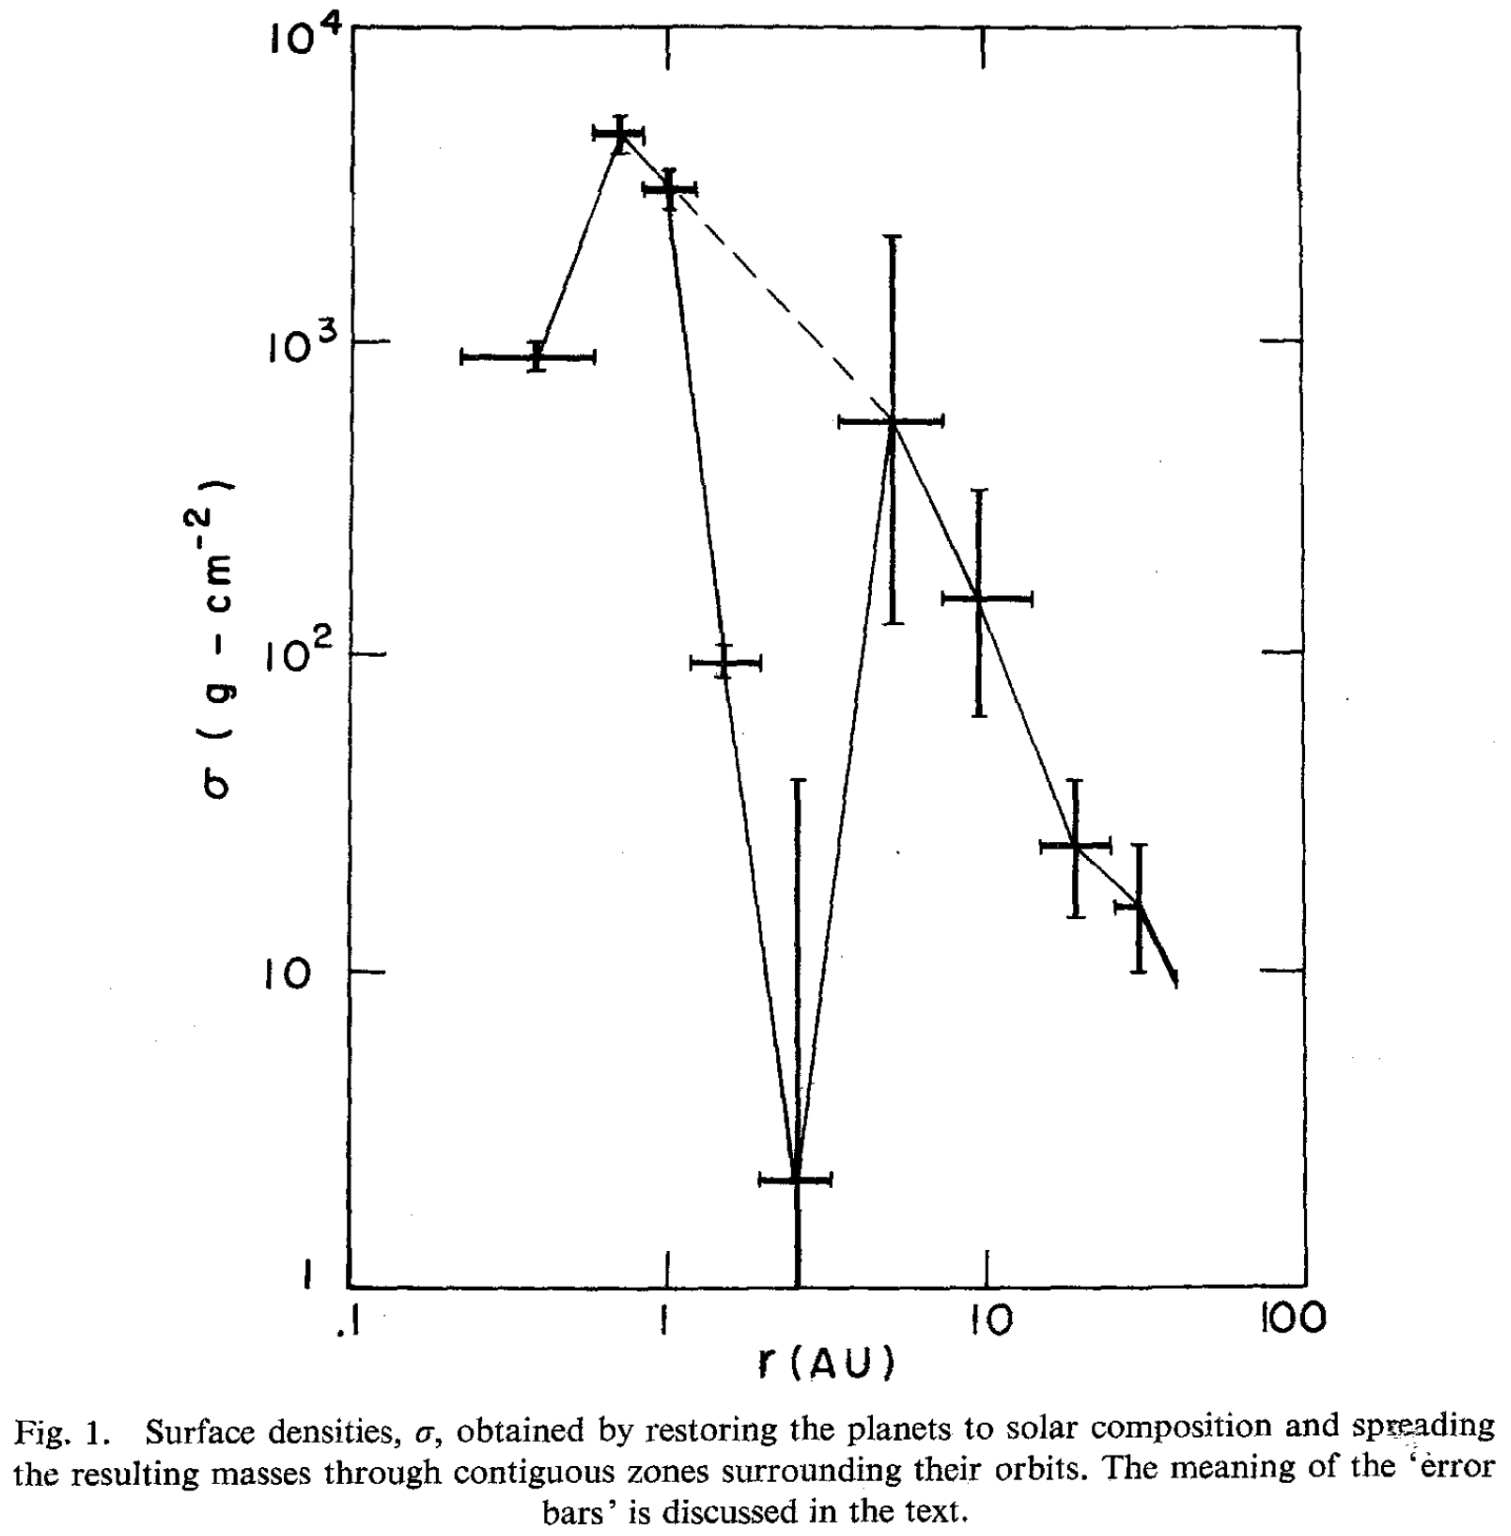
\includegraphics[trim={0cm 5cm 0 0cm},clip, width=0.9\textwidth]{Snebuladensity}\label{fig:Snebuladensity}\caption{Andamento minimum mass solar nebula (MMSN). Da \cite{weidenschilling1977distribution}.}
\end{figure}

Per stimare la massa del disco protoplanetario \cite{weidenschilling1977distribution} ha considerato la massa presente nei pianeti e nella fascia asteroidale arricchita di H/He per avere composizione solare: distribuendo questa massa in un anello di spessore proporzionale al raggio di Hill e centrato sulle orbite si ha l'andamento della densit\'a superficiale mostrato in \ref{fig:Snebuladensity}, $\sigma\propto r\expy{-3/2}$.

\begin{workout}[accrescimento di gas su nucleo solido prevede arricchimento di metalli ]

\end{workout}

La formazione per accrescimento di gas su nucleo solido prevede arricchimento di metalli rispetto alla composizione di partenza. Vincoli alla densit\'a sono imposti dalla misura dei momenti di multipolo del potenziale gravitazionale: risolvendo un modello di pianeta che rientri nei vincoli osservativi si determinano la massa del core e la metallicit\'a dell'inviluppo gassoso dei 4 pianeti gassosi (vedi  \ref{tab:JSUNcomp}).

\begin{table}[!htb]
    \begin{minipage}{.5\linewidth}
      \centering
        \begin{tabular}{ccc}
&\parbox{1.5cm}{Jupiter $317.8\mearth{}$}&\parbox{1.5cm}{Saturn $95.1\mearth{}$}\\
  $M_c$&$0-11\mearth{}$&$9-22\mearth{}$\\
$M_Z$&$1-39\mearth{}$&$1-8\mearth{}$\\
$M_Z^{tot}$&$8-39\mearth{}$&$13-28\mearth{}$\\
$Z/Z_{\odot}$&$1-6$&$6-14$\\
 \end{tabular}
    \end{minipage}%
    \begin{minipage}{.5\linewidth}
      \centering
        \begin{tabular}{ccc}
&\parbox{1.5cm}{Uranus $14.5\mearth{}$}&\parbox{1.5cm}{Neptune $17.1\mearth{}$}\\
$M_{rock}$&$3.7\mearth{}$&$4.2\mearth{}$\\
$M_{ice}$&$9.3\mearth{}$&$10.7\mearth{}$\\
$M_{H/He}$&$1.5\mearth{}$&$2.2\mearth{}$\\
        \end{tabular}
    \end{minipage} 
    \caption{Composizione Giove, Saturno, Urano e Nettuno. Da \cite{baraffe2009physical}}\label{tab:JSUNcomp}
\end{table}

Il modello di Nizza del sistema solare riproduce caratteristiche orbitali dei pianeti giganti considerando la loro migrazione in una distribuzione di planentesimi di $30-50\mearth{}$; la presenza di numerosa popolazione di planetesimi \'e corroborata dalla craterizzazionedei pianeti terrestri e corpi minori come dall'esistenza di numerosi oggetti di piccole dimensioni superstiti.

\begin{workout}[Cosa dire dei modelli planetarii: core giganti gassosi: modelli planetari e raffronto isolation mass in MMSN]
parte relativa ai momenti multipolo gravitazionale. 
In hydrostatic equilibrium the external gravitational potential is
\begin{align}
&V(r,\theta)=\frac{GM_p}{r}[1-\sum_1^{\infty}(\frac{R_+}{r})^{2n}J_{2n}P_{2n}(\theta)]\\
&J_{2n}=-\frac{1}{M_pR_+^{2n}}\int\rho(r) r\expy{2n}P_{2n}(\theta)\,d^3r
\end{align}
zharkov trubitsyn 74
\end{workout}

\begin{workout}[Earth age]
pg 297; allegre 95
\end{workout}

\begin{workout}[Planetesimal and late heavy bombardament]
pg 302
Introdurre planetesimi: migrazione.
debris disk: pg 222
Si ipotizza che i planetesimi superstiti popolino la fascia di Kuiper e la nube di Oort

\end{workout}

\begin{workout}[Stellar age: isochrone fitting]
Jorgensen Lindegren 05
\end{workout}

\begin{workout}[et\'a corpi sistema solare (age and chronology)]
age of the sun: $4.57Gyr$ (Bahcall95)
CAI: $4567Gyr$ +3Myr chondrule
\end{workout}

\begin{workout}[Sistema solare - andamento densit\'a e composizione]
asteroid mercury mars mass depletion pg 298
farinella pg513,weidenschilling 77,

\end{workout}

\begin{workout}[atmospher composition and photoevaporation]
pg 256: interior and atmosphere, 293 solar system, 143 properties of transit
\end{workout}


\begin{workout}[Noble gas enrichment]
FORMATION OF GIANT PLANETS ? AN ATTEMPT IN MATCHING OBSERVATIONAL CONSTRAINTS
\end{workout}

\begin{workout}[Degree of super-adiabaticity: Struttura interna (assimption for pre-runaway accretion)]
See: characterization of exoplanets from their formation (pg4)
Degree of super-adiabaticity: baraffe 02, Rafikof 07
\end{workout}

\begin{workout}[few well separeted homogeneous region: Struttura interna (assimption for pre-runaway accretion)]
See: characterization of exoplanets from their formation (pg4)
Baraffe 07: composition gradients, core dissolution: Wilson, Militzer 12, planetesimal deconstruction: mordasini 05, multiconvective layers: Leconte chabrier 12.
\end{workout}

\begin{workout}[Full packing/spacing]

\end{workout}

\begin{workout}[Orbit of terrestrial planets]
Constrain for core accretion model ofgiant planets: dynamical shakeup Nagasawa 05 Thommes08c
\end{workout}

\begin{workout}[Earth post-oligarchic growth]
perryman pg229
\end{workout}


\begin{workout}[Planetesima migration: pluto eccentricity, large population of Kuiper belt object]

\end{workout}

\begin{workout}[Planet obliquity:]
Schlichting sari 07: The effect of Semi-Collisional Accretion on Planetary Spins
Inconsistent with isotropic distro (Tremaine 1991). Randomly directed component of spin angular momentum (Kokubo Ida 07) cause large then observed i,e (Harris Ward 82).
Planetesimal/protoplanet collision would imply stachastic rather than smooth accretion.
Excittion of giant planet spin obliquity if spin axis precession freq pass through resonance with orbital prec freq during migration.
Uranus: tilt due to collision or migration: Bergstralh 91 or Bou\'e Laskar 10.
Non of obliquity of terrestrial planet are belived primordial (secular orbit perturbation)+tidal dissipation.
Effects of inhomogenous infall on obliquity (tremaine 91, bate 10)
\end{workout}


{\let\clearpage\relax\let\cleardoublepage\relax
\chapter{Caratteristiche della popolazione di esopianeti}
}

\begin{wrapfigure}[5]{l}{0.55\textwidth}
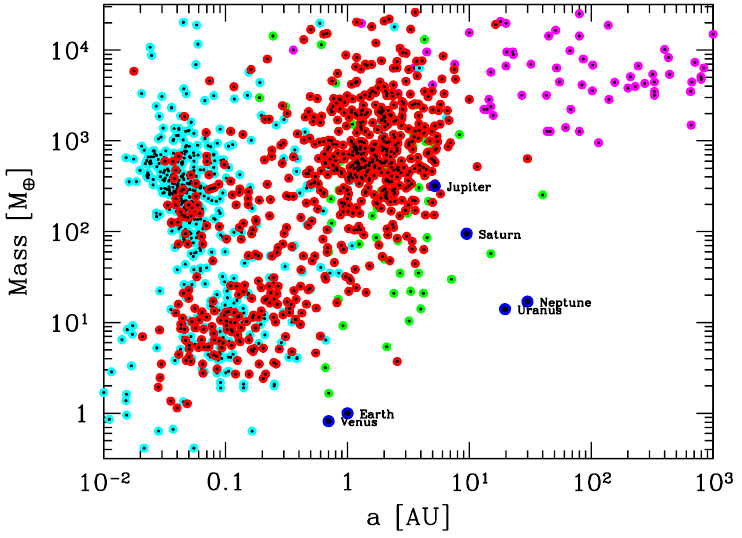
\includegraphics[trim={0cm 0 0 0},clip, width=0.5\textwidth]{obsMa}\label{fig:Maplot}
\caption{Diagramma massa-distanza degli esopianeti in ''The extrasolar planet encyclopedia''. Rosso, celeste, magenta e verde sono pianeti rivelati tramite RV, T, osservazione diretta e microlensing. Da \cite{mordasini2018}.}
\end{wrapfigure}

La popolazione degli esopianeti osservata riflette quella reale tramite gli effetti di selezione dovuti alla probabilit\'a di rivelamento della tecnica/strumento particolari. Le osservazioni pi\'u numerose sono basate sull'osservazione della velocit\'a lungo la linea di vista dovuto al moto della stella attorno al baricentro del sistema stella pianeta (RV) o differenza nella luminosit\'a dovuto al transito del pianeta tra stella e osservatore (T).

\begin{workout}[bimodal radius distro is observed by transit?]
Characterization of exoplanets from their formation II. The planetary mass-radius relationship pg 21: bimodal radius distribution
\end{workout}

\begin{workout}[frequenza sistemi planetarii:doppler + transito]
tab.1 mayor11(RV)
tab.1: occurrence and architecture exoplanetary system 
\end{workout}

\begin{workout}[Occurence rate]
\begin{itemize}
\item Coralie hot jupiter: giant planets $M\sin{i}>0.2\mjupiter$ and $a<0.1au$; $5.6\%$ giant out to 4au
\item Lick/Keck/AAT ($M\sin{i}>0.5\mjupiter$): $1.2\%$ stars have hot jupiter and $6.6\%$ giant within 5 au
\item ...
\end{itemize}•
\end{workout}

\section{Popolazione esopianeti rilevati tramite RV}

Se l'asse z \'e lungo la linea di vista la posizione della stella \'e $z=r(t)\sin{i}\sin{(\omega+\nu)}$ e per la velocit\'a radiale:
\begin{align}
&v_r=\dot{z}=K[\cos{(\omega+\nu)}+e\cos{\omega}]\label{eq:vrsignal}\\
&K=\frac{2\pi}{P}\frac{a_*\sin{i}}{(1-e^2)\expy{1/2}}=(\frac{2\pi G}{P})\expy{1/3}\frac{M_p\sin{i}}{(M_p+M_*)\expy{2/3}}\frac{1}{(1-e^2)\expy{1/2}}
\end{align}
dove $K$ \'e la semi-ampiezza.
Per probabilit\'a di rivelamento del $50\%$ la minima massa planetaria \'e
\begin{equation}
M_{p,min}\approx4\mearth{}(\frac{N}{20})\expy{-1/2}(\frac{\sigma}{\SI{1}{\meter\per\second}})(\frac{P}{\SI{1}{\day}})\expy{1/3}(\frac{M_*}{\msun{}})\expy{2/3}
\end{equation}
dove $\sigma$ tiene conto errori strumentali e rumore stellare.

Per sistemi multipli consideriamo la sovrapposizione lineare di $n_p$ termini \eqref{eq:vrsignal}: viene sottratto il segnale Kepleriano dominante fino a che resta solo rumore.

\begin{figure}[!ht]
\begin{subfigure}[b]{0.49\textwidth} \centering 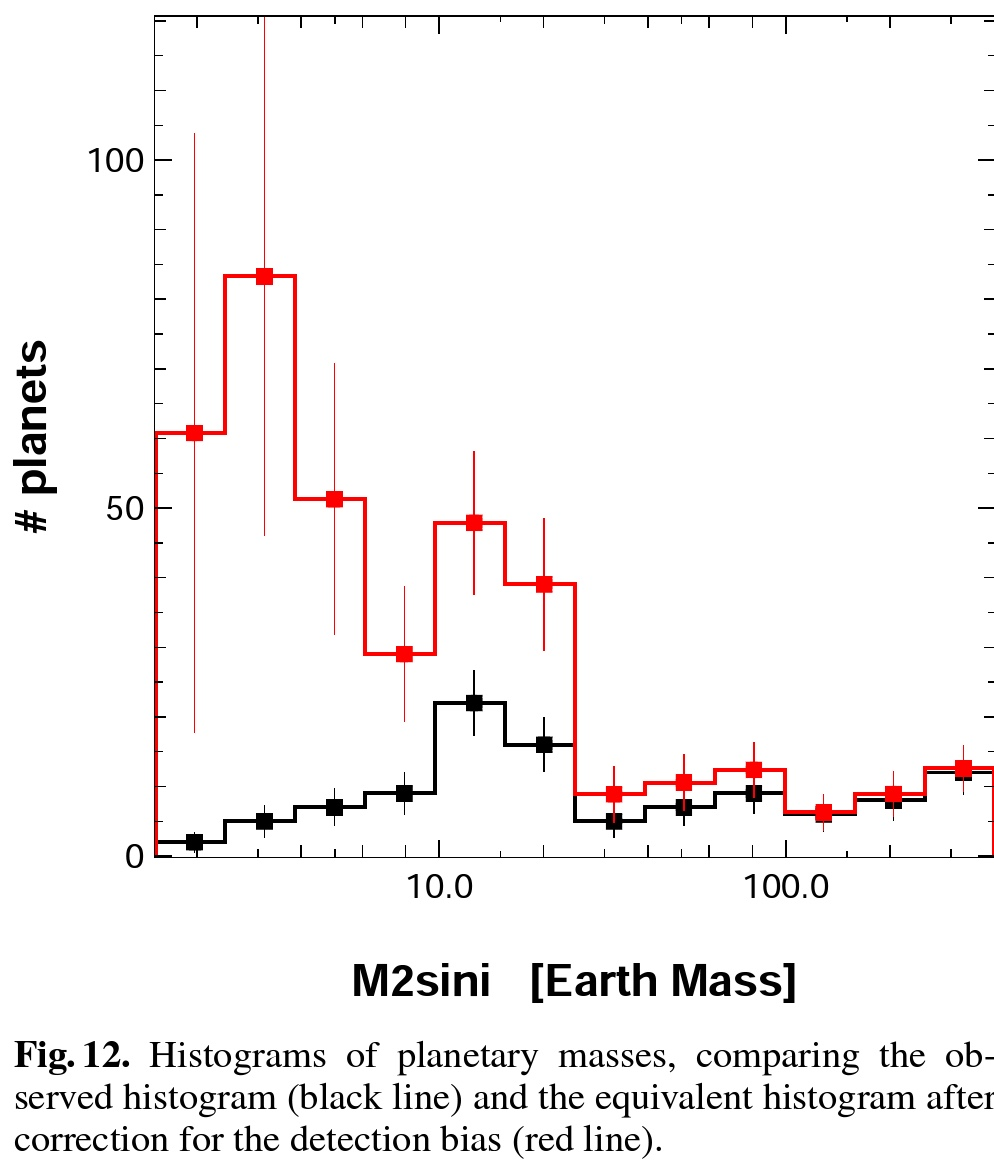
\includegraphics[trim={0cm 5cm 0 0},clip, width=0.94\textwidth]{freqvsM}
\caption{Distribuzione di massa di massa dei pianeti: in rosso distribuzione corretta per bias osservativi. Da \cite{mayor2011harps}.}\label{fig:freqvsM} \end{subfigure}
~
\begin{subfigure}[b]{0.49\textwidth} \centering 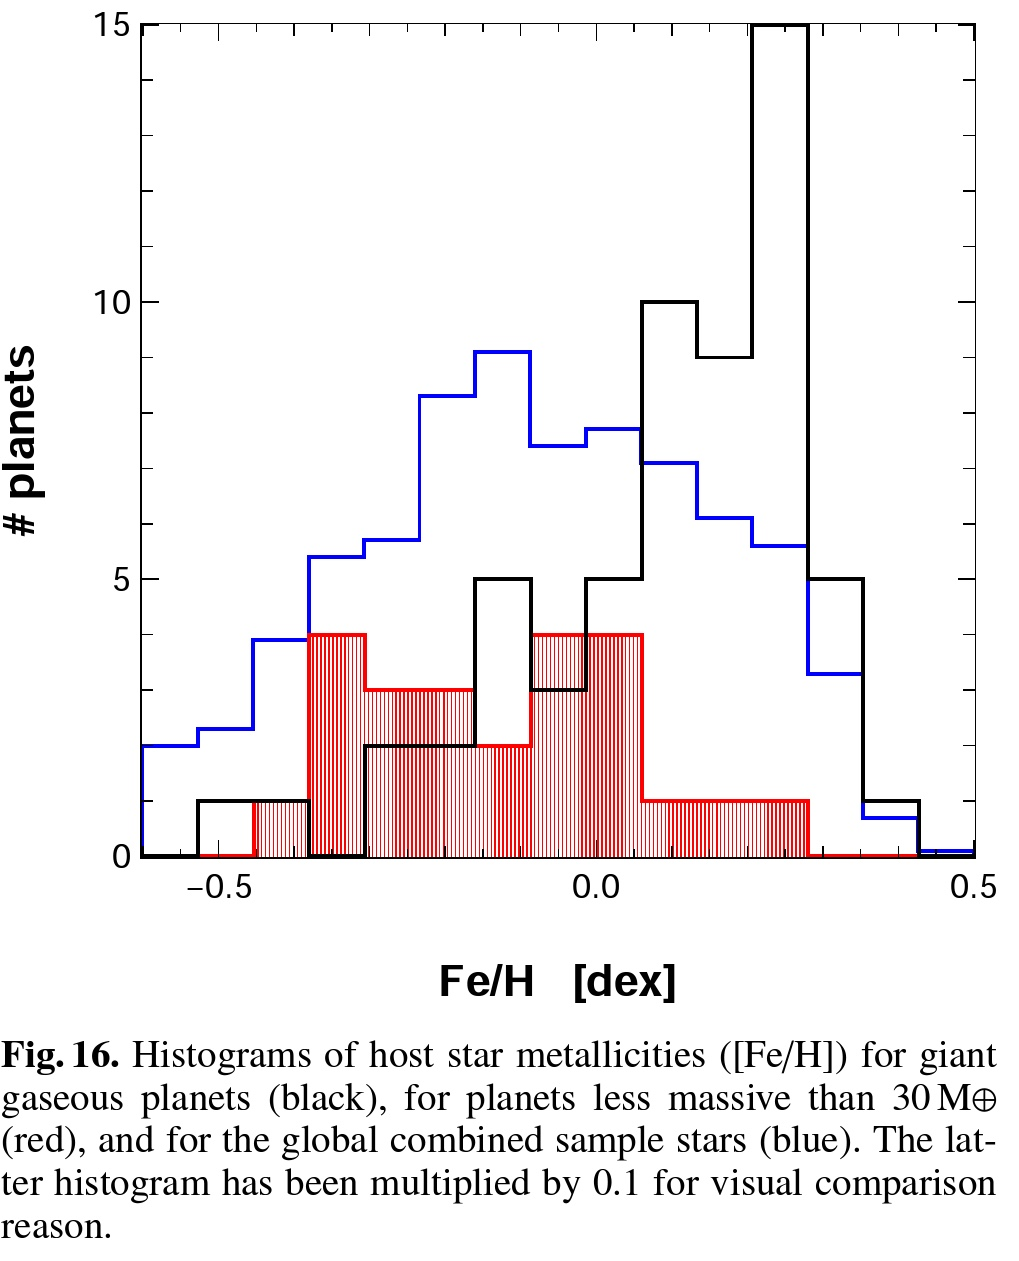
\includegraphics[trim={0cm 8cm 0 0},clip, width=0.94\textwidth]{PfreqvsFeH}\label{fig:PfreqvsFeH}
\caption{Numero di pianeti in funzione della metallicit\'a stellare: nero dei giganti gassosi, rosso dei pianeti con $M\leq30\mearth{}$ e blu combinata. Da \cite{mayor2011harps}}
\end{subfigure}
\end{figure}

La distribuzione di massa (\ref{fig:freqvsM}) mostra un'abbondante popolazione di pianeti di massa piccola e una rapida diminuzione attorno a $10\mearth{}$; la distribuzione dei periodi mostra aumento dei pianeti giganti ($M>30\mearth{}$) a maggiore periodo orbitale e concentrazione pianeti piccola massa a $P=10-100\si{\day}$.

La \ref{fig:freqZstar} mostra l'assenza di correlazione tra la metallicit\'a della stella e la frequenza di pianeti di piccola massa fino a $30-40\mearth{}$ al contrario di quello che accade per pianeti giganti.

\begin{figure}[!ht]
\begin{subfigure}[b]{0.49\textwidth} \centering 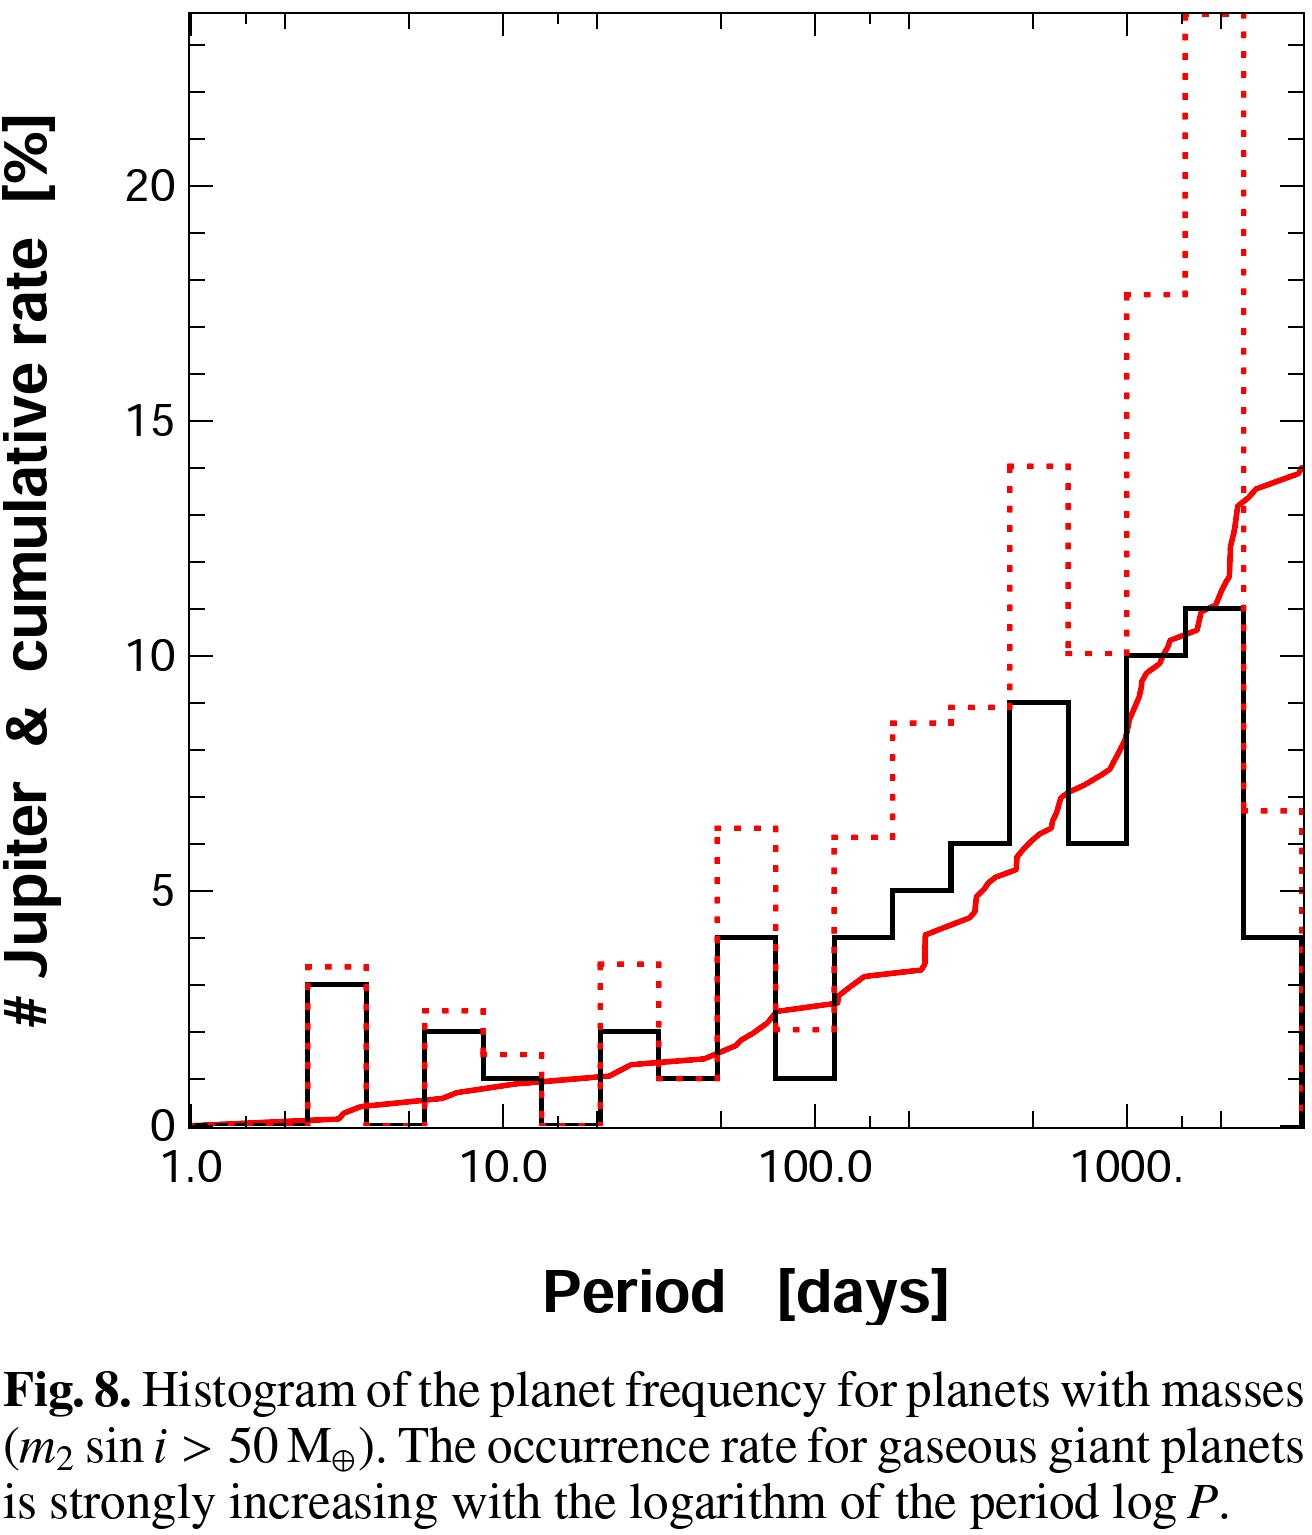
\includegraphics[trim={0cm 6cm 0 0},clip, width=0.98\textwidth]{freqvsPgiant}\caption{Frequenza pianeti con $M\geq 30\mearth{}$ in funzione del periodo orbitale; in rosso  tratteggiato con correzione bias osservativi. Da \cite{mayor2011harps}.}\label{fig:freqvsPgiant} \end{subfigure}
~
\begin{subfigure}[b]{0.49\textwidth} \centering 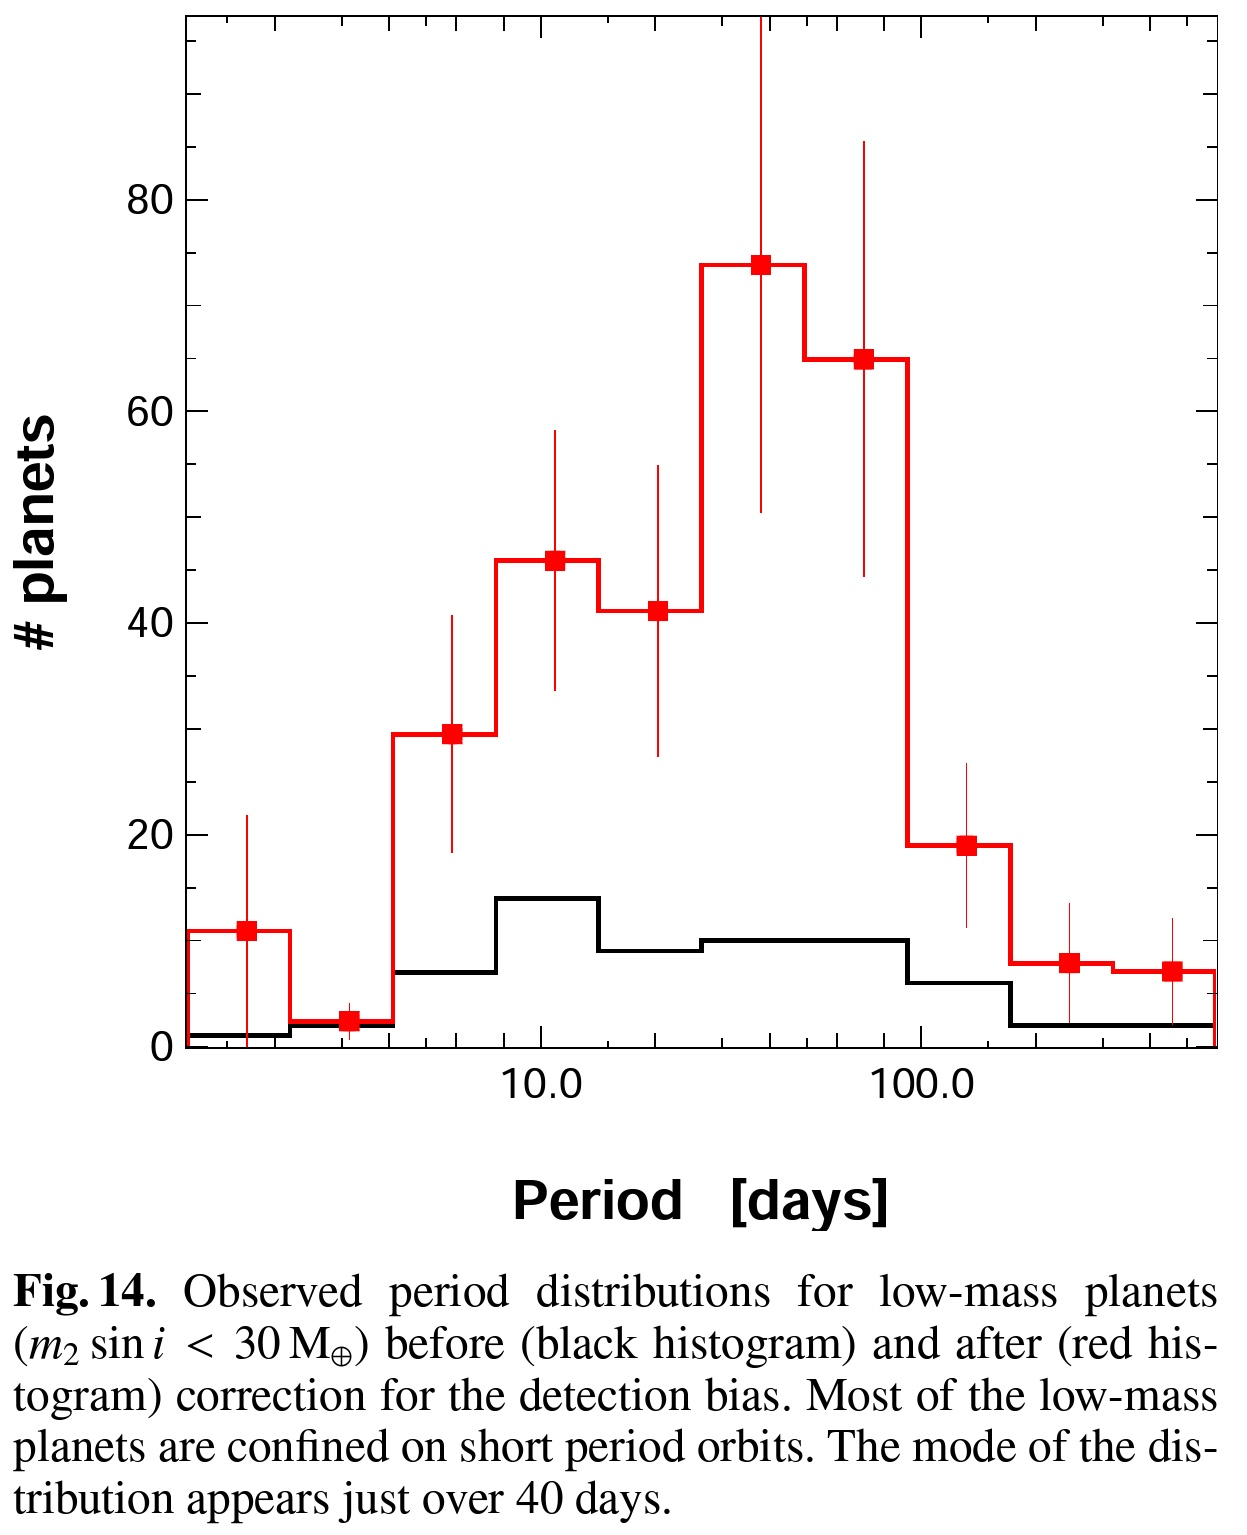
\includegraphics[trim={0cm 10cm 0 0},clip,width=0.98\textwidth]{freqvsPlowM}\label{fig:freqvsPlowM} \caption{Frequenza pianeti con $M\leq 30\mearth{}$ in funzione del periodo orbitale; in rosso con correzione bias osservativi. Da \cite{mayor2011harps}.}
\end{subfigure}
\end{figure}

\begin{figure}[!ht]
\begin{subfigure}[b]{0.3\textwidth}
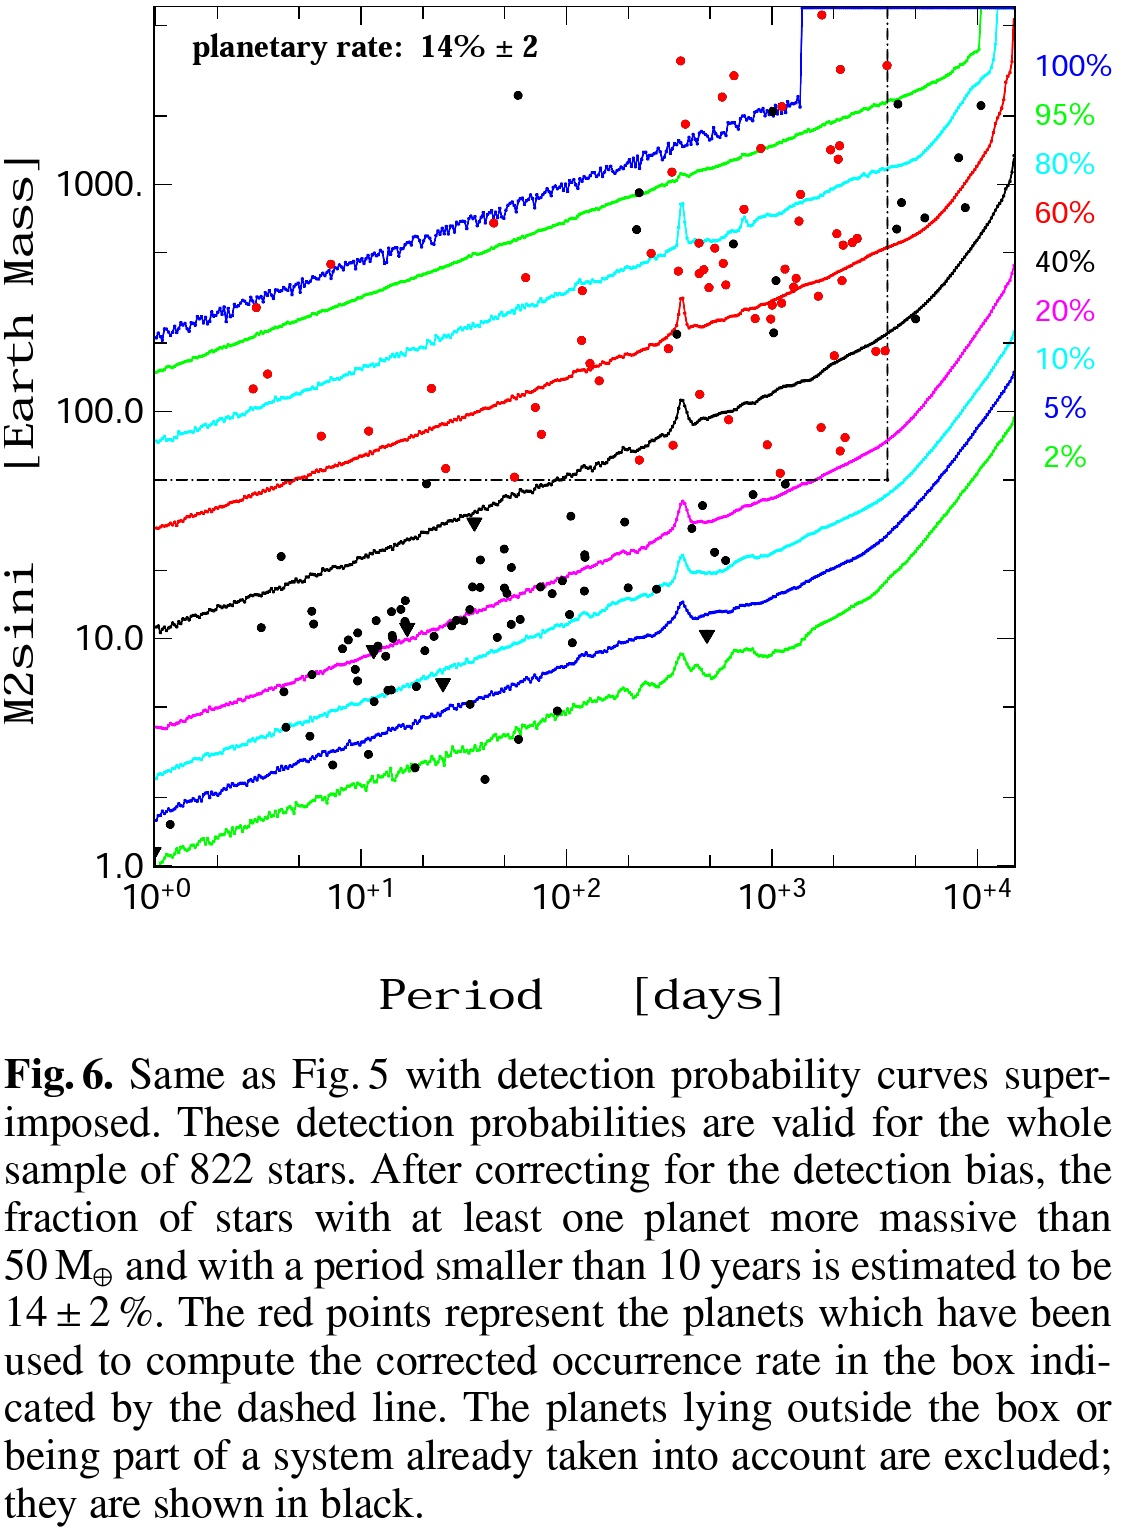
\includegraphics[trim={0cm 17cm 0 0},clip, width=0.9\textwidth]{PMfreq-e23}\label{fig:PMfreq-e23}
\end{subfigure}
~
\begin{subfigure}[b]{0.3\textwidth}
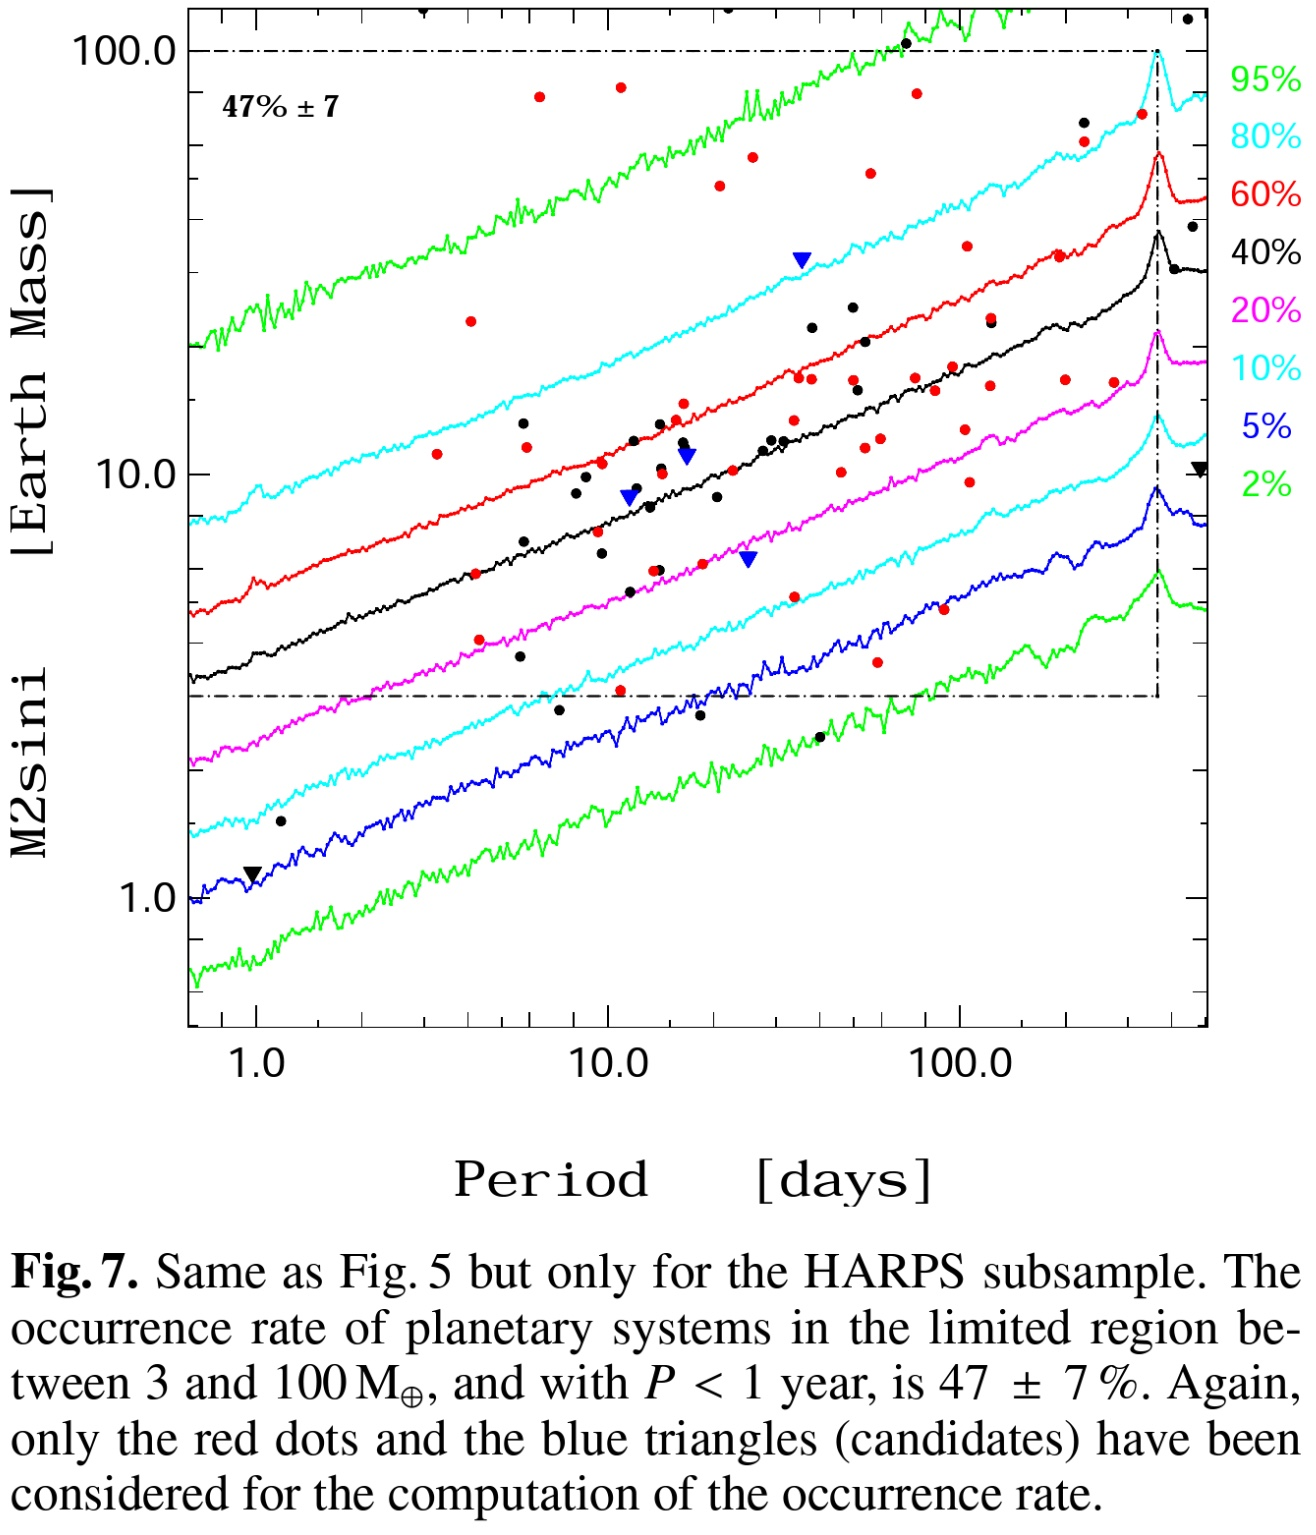
\includegraphics[trim={0cm 10cm 0 0},clip, width=0.9\textwidth]{PMfreq-e12}\label{fig:PMfreq-e12}
\end{subfigure}
~
\begin{subfigure}[b]{0.3\textwidth}
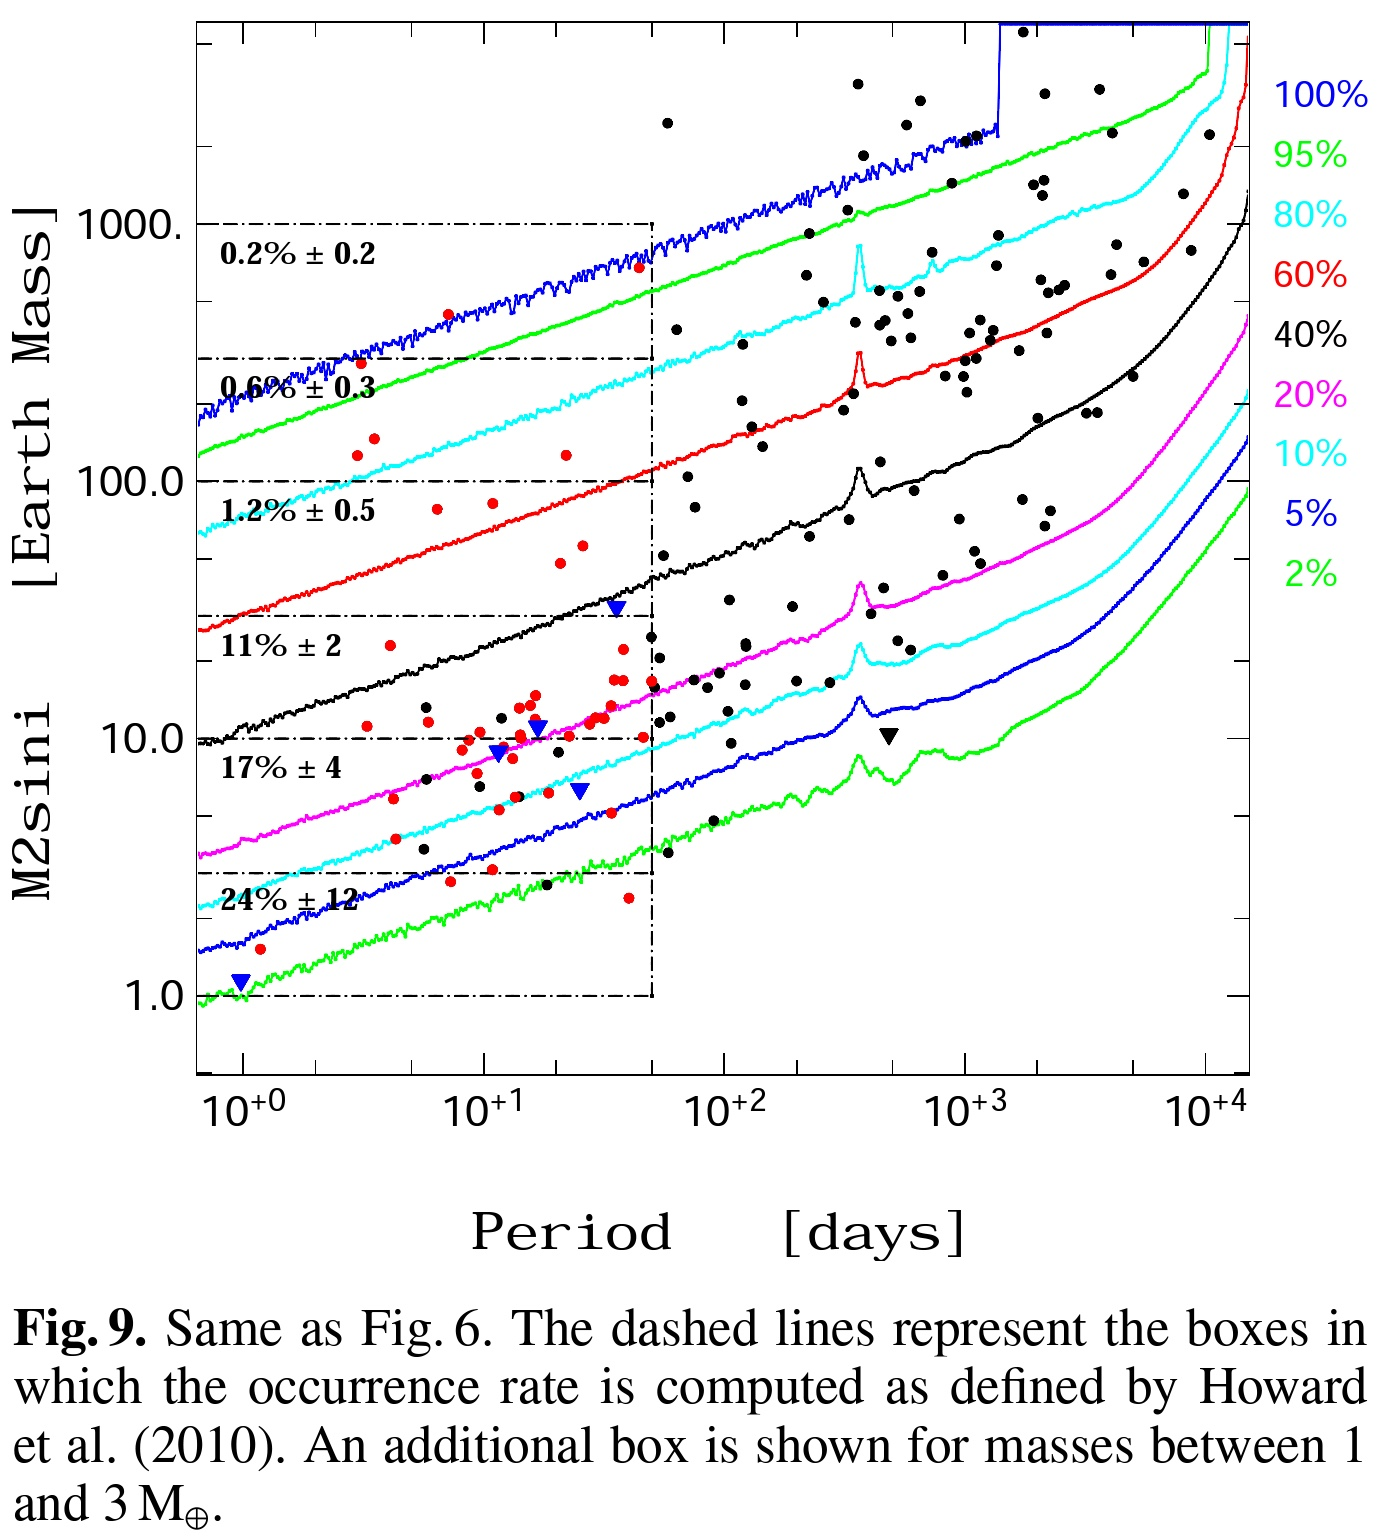
\includegraphics[trim={0cm 8cm 0 0},clip, width=0.9\textwidth]{PMfreq-short}\label{fig:PMfreq-short}
\end{subfigure}
\caption{Diagramma massa-periodo: frazione di stelle che ospitano pianeta con caratteristiche nella regione evidenziata. Da sinistra a destra: $P<10\si{\year}$ e $M>50\mearth{}$, $P<1\si{\year}$ e $M>3-100\mearth{}$, $P<50\si{\day}$ e $M=1-3/3-10/10-30/30-100/100-300/300-1000$. Da \cite{mayor2011harps}}
\end{figure}

Una comprensione pi\'u ampia si ha studiando la distribuzione dei pianeti nel diagramma massa-periodo (M-P): elenco alcune caratteristiche della distribuzione dei pianeti osservati (da \cite{mayor2011harps}).
\begin{itemize}
\item Il picco della densit\'a di super-terre si sposta da $6\mearth{}$ a $10\mearth{}$ per periodi da \SI{10}{\day} a \SI{100}{day}
%\item Non sono osservati pianeti fino a $50\mearth{}$ con $P>\SI{1000}{\day}$
\item il pianeta gassoso pi\'u massiccio aumenta da $1\mjupiter{}$ a $15\mjupiter{}$ passando da $P\approx\SI{1}{\day}$ a $P\approx\SI{15}{\year}$.
\end{itemize}

\begin{workout}[Origin of metallicity excess: stellar structure]
Pinsonneault depoy caffee 01
\end{workout}•

\begin{workout}[minimo in mass distro]
\'e un minimo? ha un significato?
\end{workout}

\begin{workout}[dtectability and selection effects (pg 14)]
Perrymann pg 34 fig 2.25 d
fig 2.6,fig 2.18
\end{workout}

\begin{workout}[multplanet system: mean motion resonances, orbital spacing,...]
dynamical classification (barnes 08): tidal dominated if ($a<0.1$), resonant dom. if one resonant argument librates, secular otherwise.
Many systems are found dyn full and stability: packed planetary system hypothesis (Barnes Quinn 04, Barnes Raymond 04, Raymond Barnes 05, Raymond 06), orbital stability for closely packed (smith lissauer 09), outer solar system is very stable and dyna full (Levinson duncan 93, inner is less stable but dyna full (sussman wisdom 92, laskar 94)
n-body integration-orbit fitting: deprojected mass and relative inclination
perryman pg 38
Interazione n-body protopianeti vs evoluzione a lungo termine: i pianeti arrivano a risonanze attraverso migrazione
Kepler: latham 11 (first comparison of kepler planet), burke 14
wright09: ten multiplanet sysytem and systematic
Winn, Fabricky 15
fig 2.30 pg 39 Perrymann
(ford rasio 08: dynamical outcomes of PP scattering)

\begin{figure}[!ht]
\begin{subfigure}[b]{0.47\textwidth}
\centering
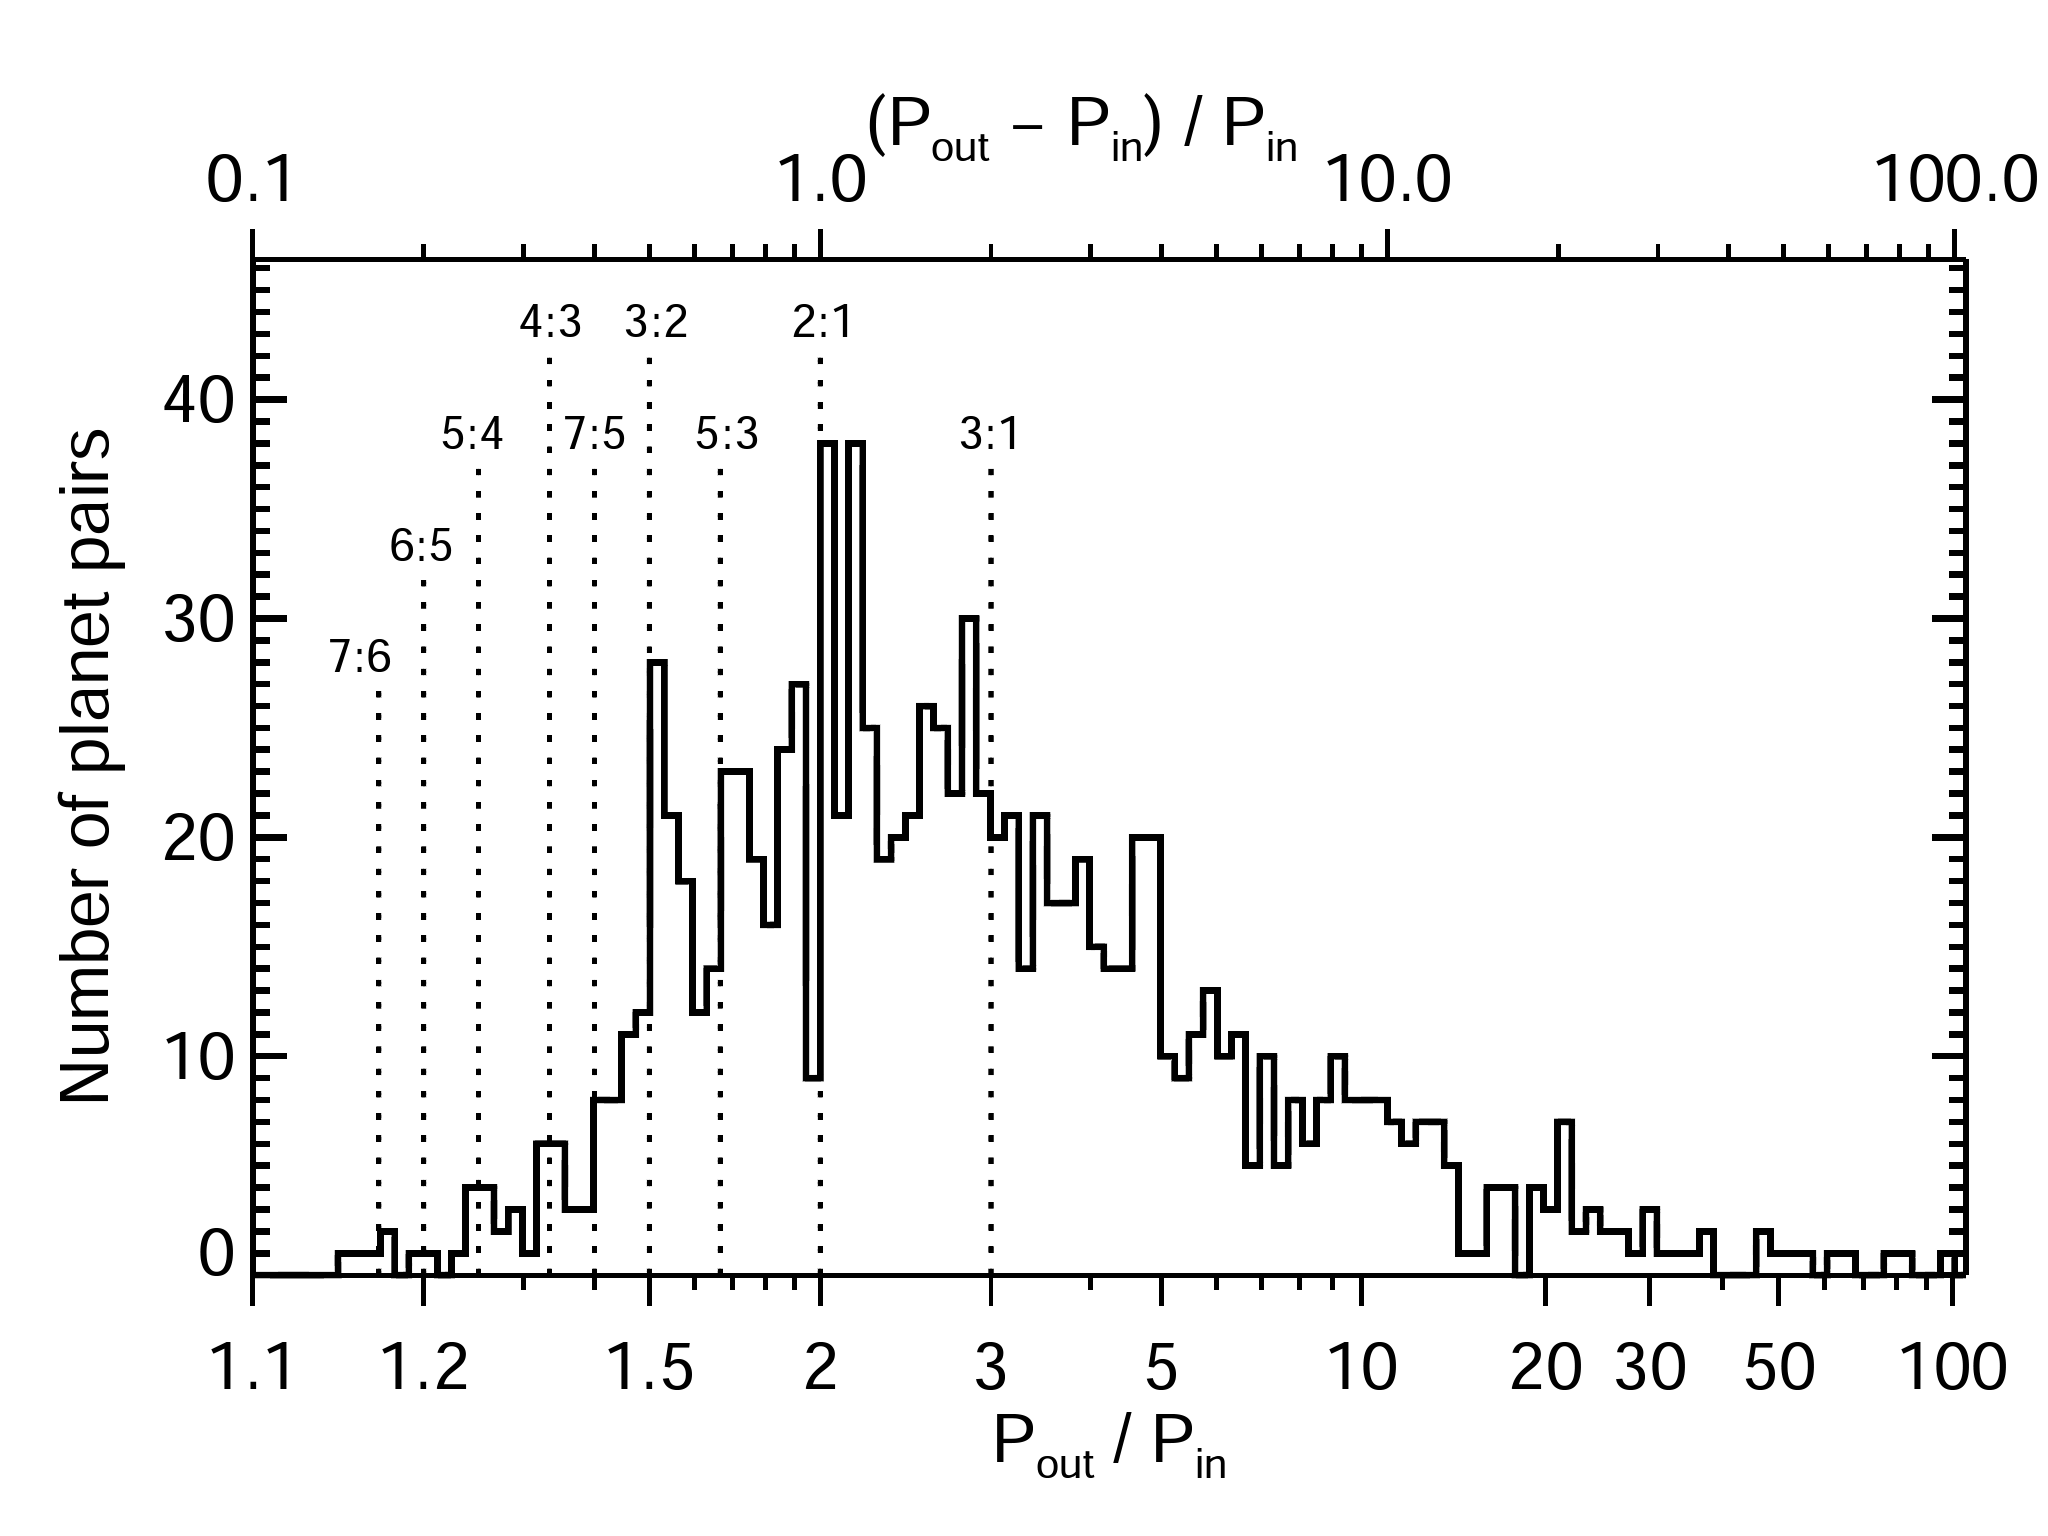
\includegraphics[trim={0cm 0 0 0},clip, width=0.9\textwidth]{exoresonance}
\caption{Da \cite{winnfabrycky15}}\label{fig:exoresonance}
\end{subfigure}
~
\begin{subfigure}[b]{0.47\textwidth}
\centering
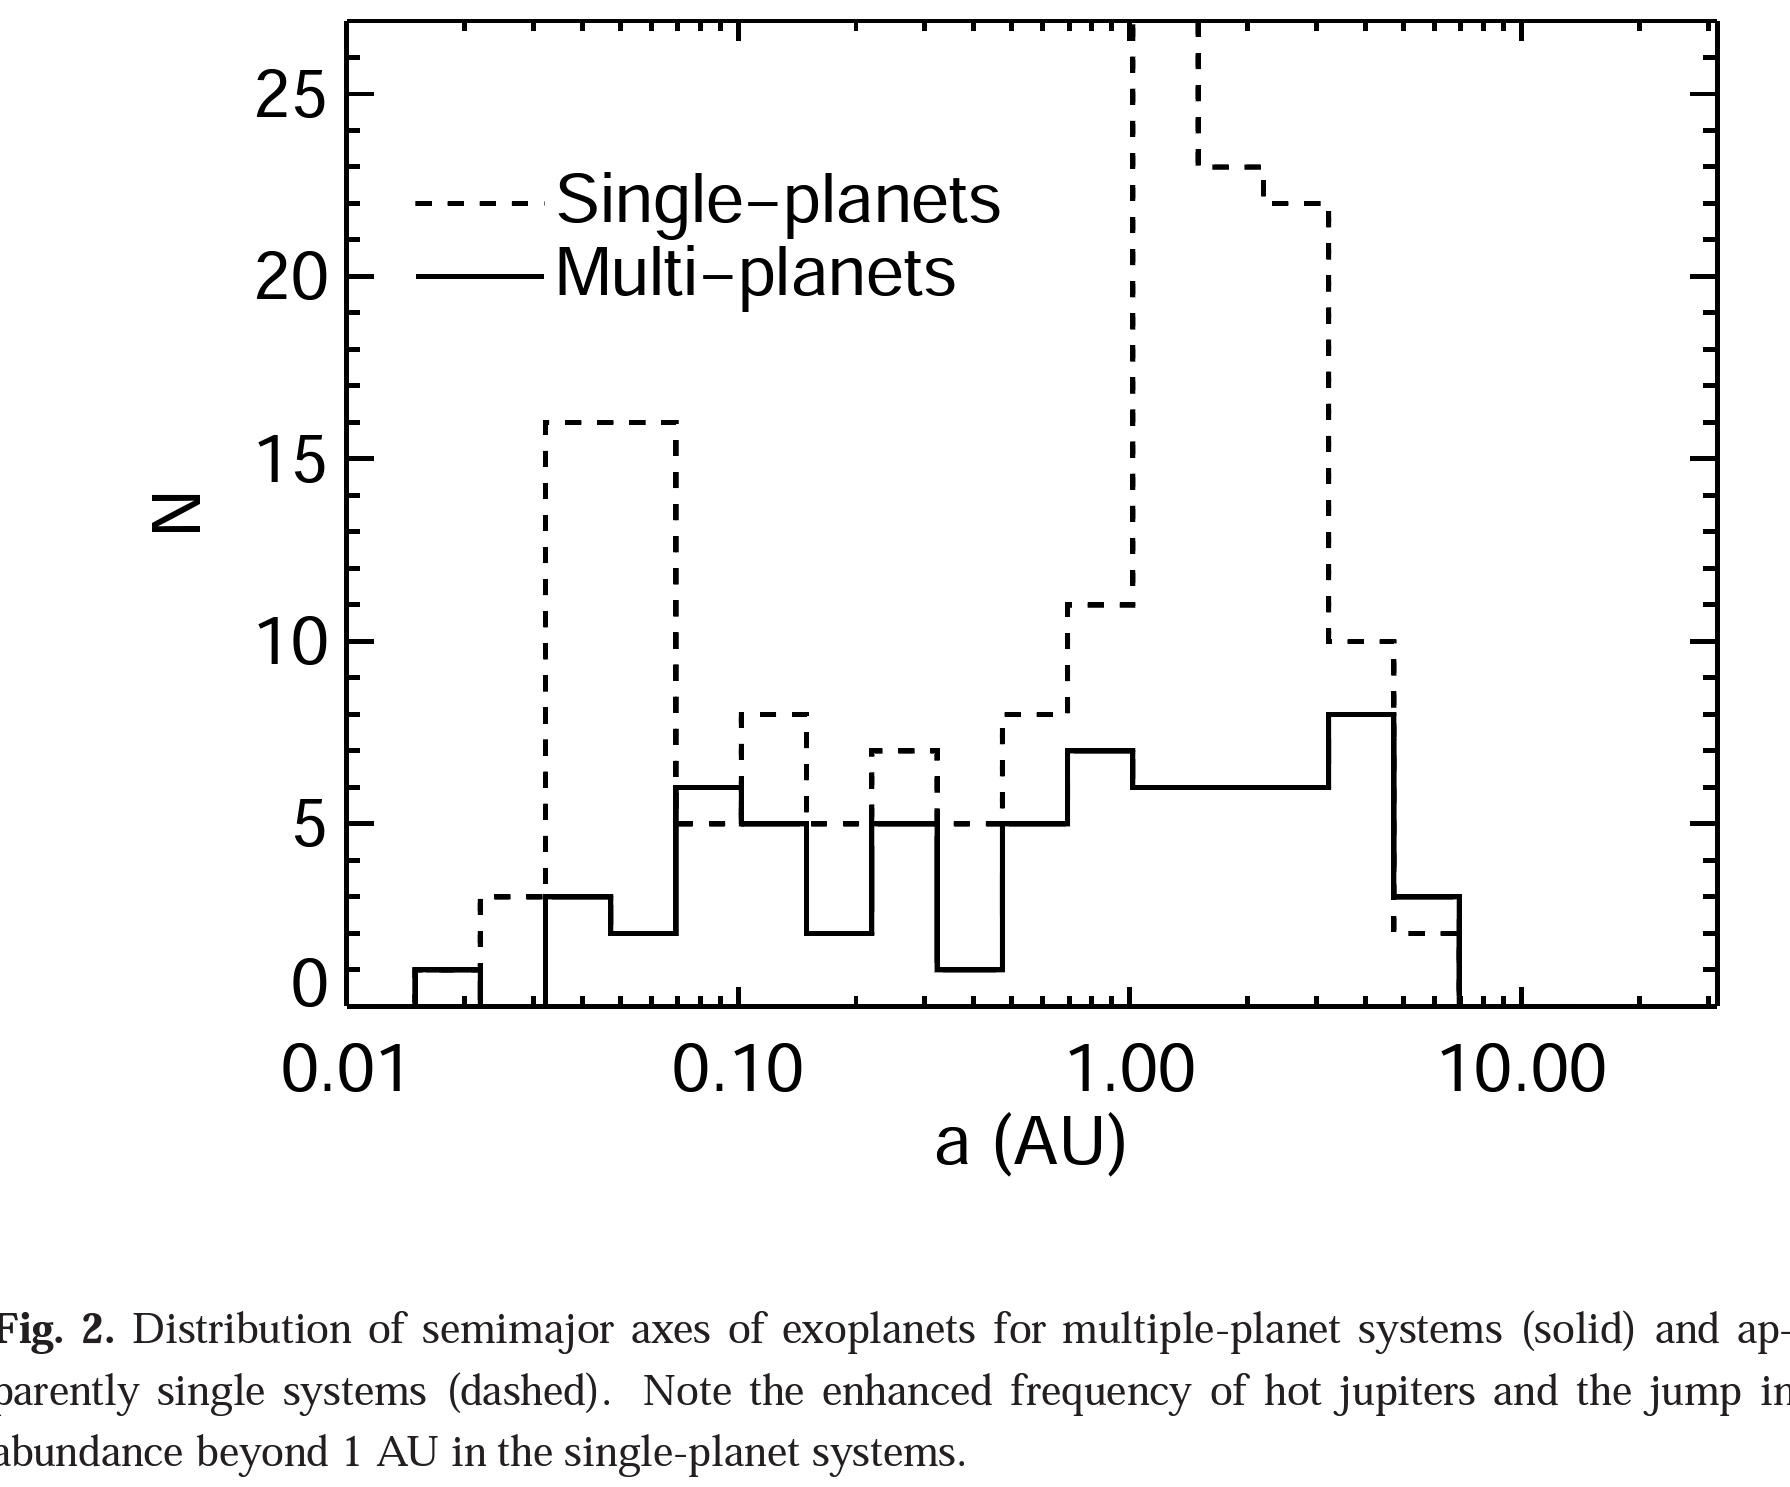
\includegraphics[trim={0cm 0 0 0},clip,width=0.9\textwidth]{singlemulti}\label{fig:}
\caption{Da \cite{wright09}}
\end{subfigure}
\end{figure}
\end{workout}

\begin{workout}[eccentricity distro: occurrence and architecture]
wright 09: multiplanet system tend to havelower eccentricity,
Limbach turner 14: $e_m\propto N\expy{-1.2}$.
planet around metal rich star have higher e (dawson, murray-clay 13)
smaller planets tend to have lower e (hogg 10 raccomanded modelling e distro on basis of Bayesian analysis)
\end{workout}

\clearpage

\section{Popolazione esopianeti rilevati tramite transito}

Le osservabili sono la differenza di luminosit\'a durante il transito, la durata totale e di massima occultazione del transito, e il periodo: da questi \'e possibile ricavare $R_p$, a, i, $R_*$, e facendo uso della relazione massa raggio appropriata per la fase evolutiva della stella $M_*$

La probabilit\'a che l'orbita di un pianeta sia allineata con l'osservatore in maniera da avere un transito, per orbite circolari ed eccentriche, \'e:
\begin{align*}
&p=\frac{R_*}{a}=0.005(\frac{R_*}{\rsun{}})(\frac{a}{1AU})\expy{-1}\\
&p=(\frac{R_*\pm R_p}{a})(\frac{1}{1-e^2})
\end{align*}
La maggiore probabilit\'a di osservazione per orbite eccentriche \'e compensata approssimativamente dalla minore durata del transito.

\begin{workout}[transiti: dectability and selection effects]
Considerando un numero totale di osservazioni $N_o$ durante il transito si hanno $N_t\approx N_o\frac{R_*}{\pi a}$; il rapport segnale rumore \'e $S/N=\sqrt{N_t}\frac{\delta}{\sigma}$, $\sigma$ precisione fotometrica, $\sigma\propto\frac{1}{\sqrt{N_{ph}}}\propto d$. Per fissato S/N e tipo stellare il numero di pianeti rivelati varia come
\begin{equation}
V_p*P\propto d^3*\frac{R_*}{a}\propto R_p^6/P\expy{\frac{5}{3}}
\end{equation}
\end{workout}


%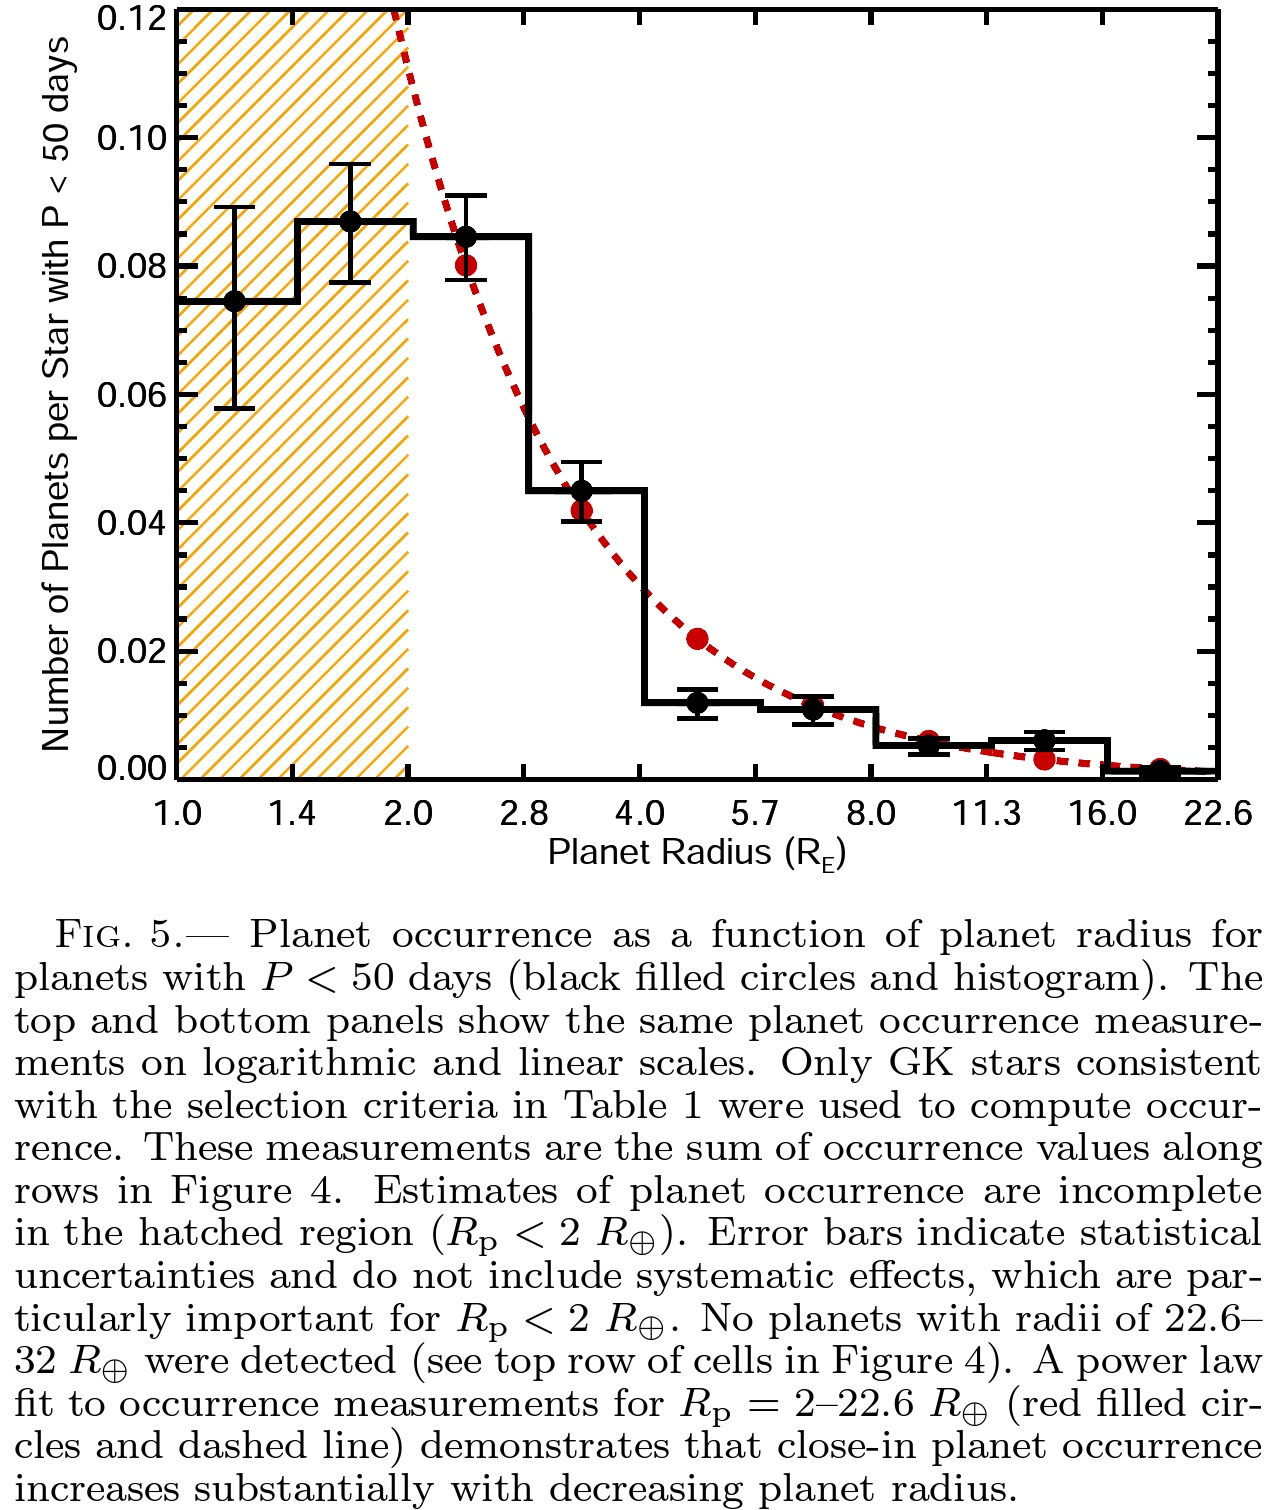
\includegraphics[trim={0cm 0 0 0},clip, keepaspectratio,width=0.9\textwidth]{freqvsRpl50d}\label{freqvsRpl50d}\caption{Da \cite{howard2012planet}}
% 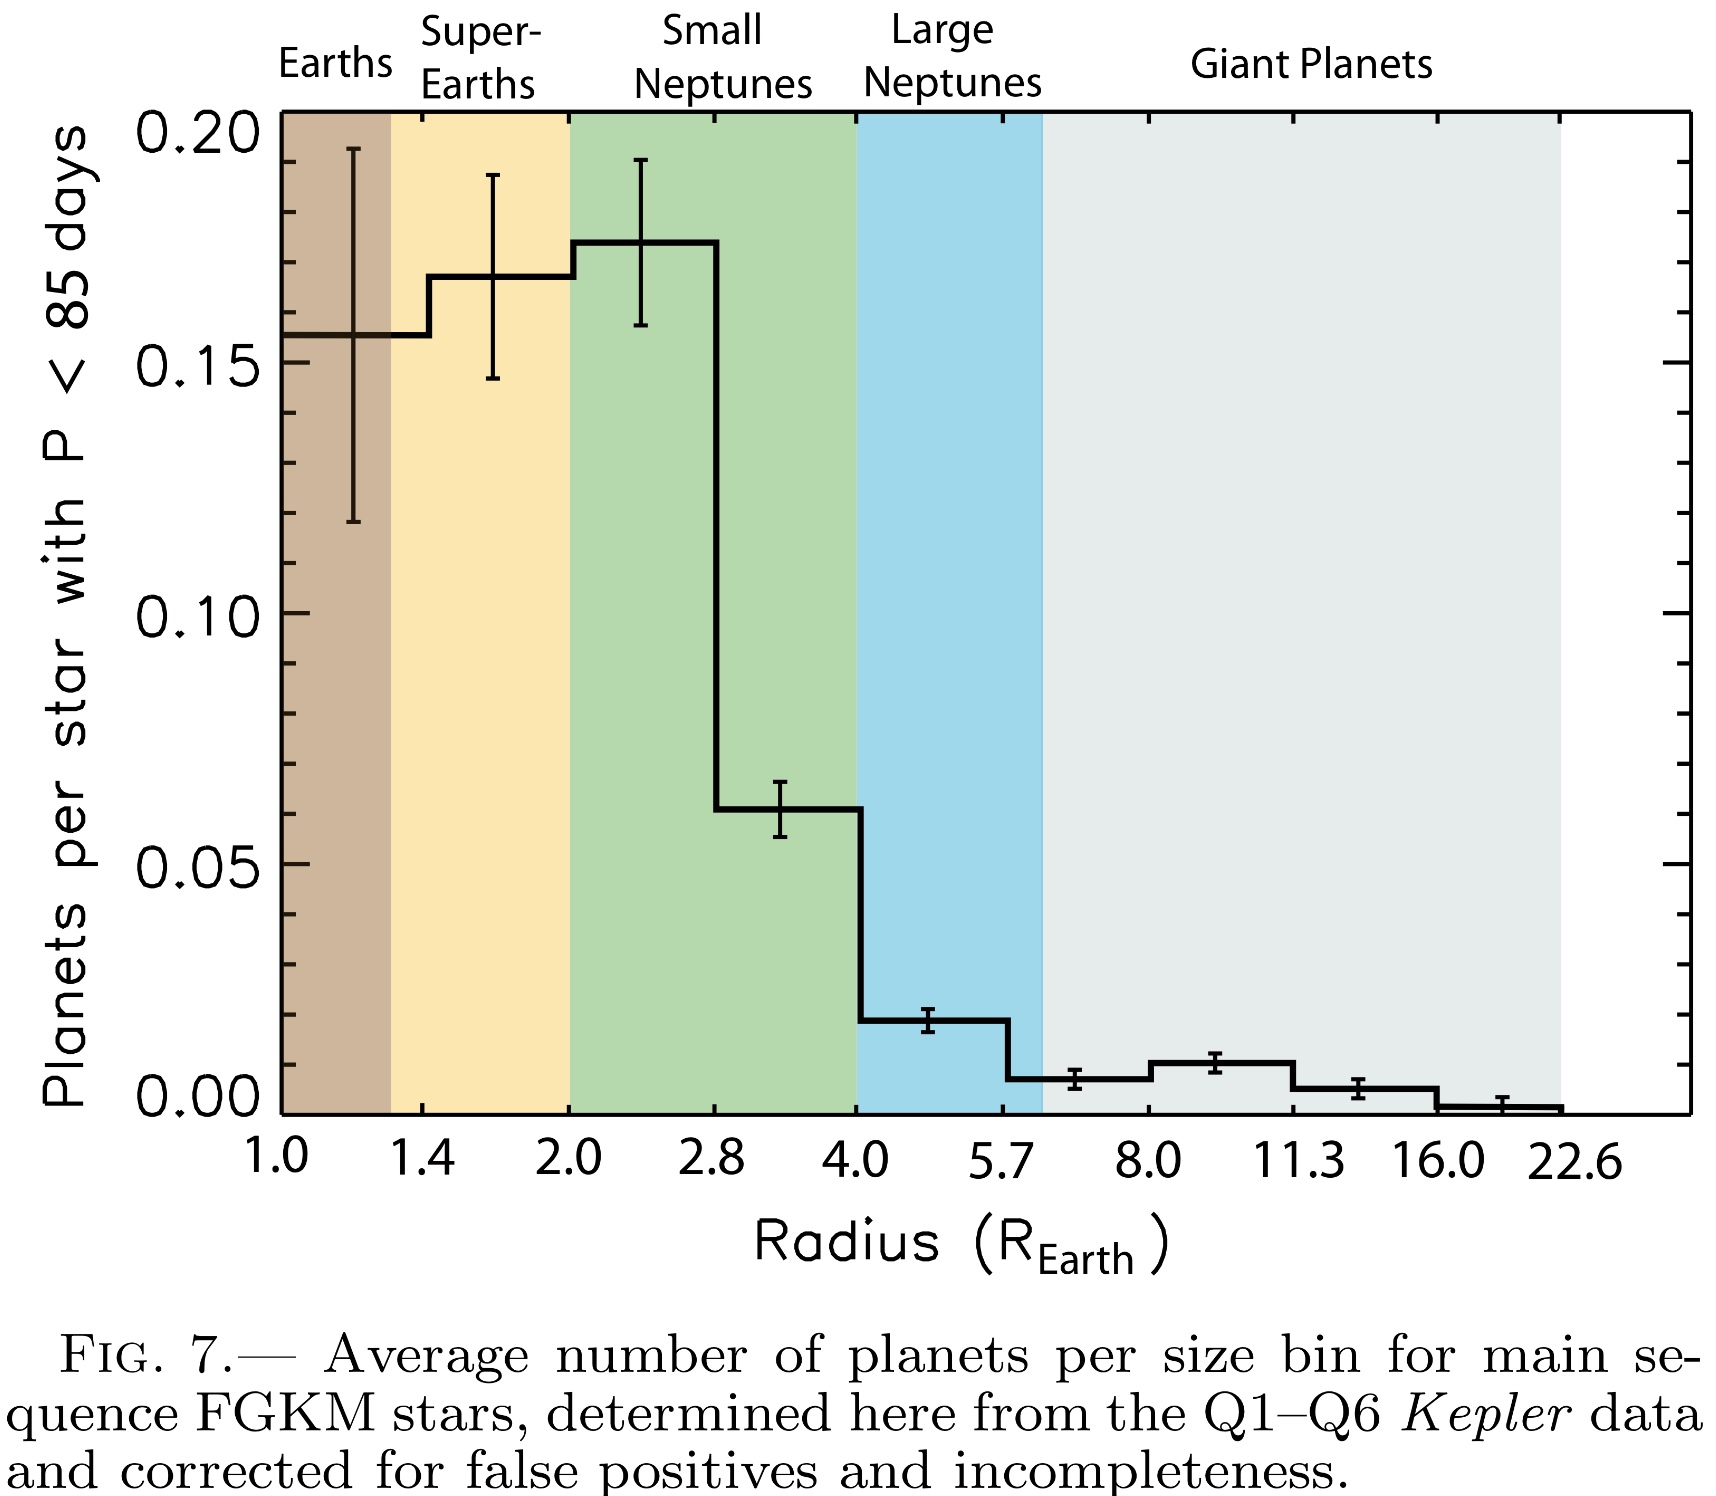
\includegraphics[trim={0cm 0 0 0},clip,width=0.95\textwidth]{keplerRfreq}\label{fig:keplerRfreq} \caption{Da \cite{fressin2013false}}
%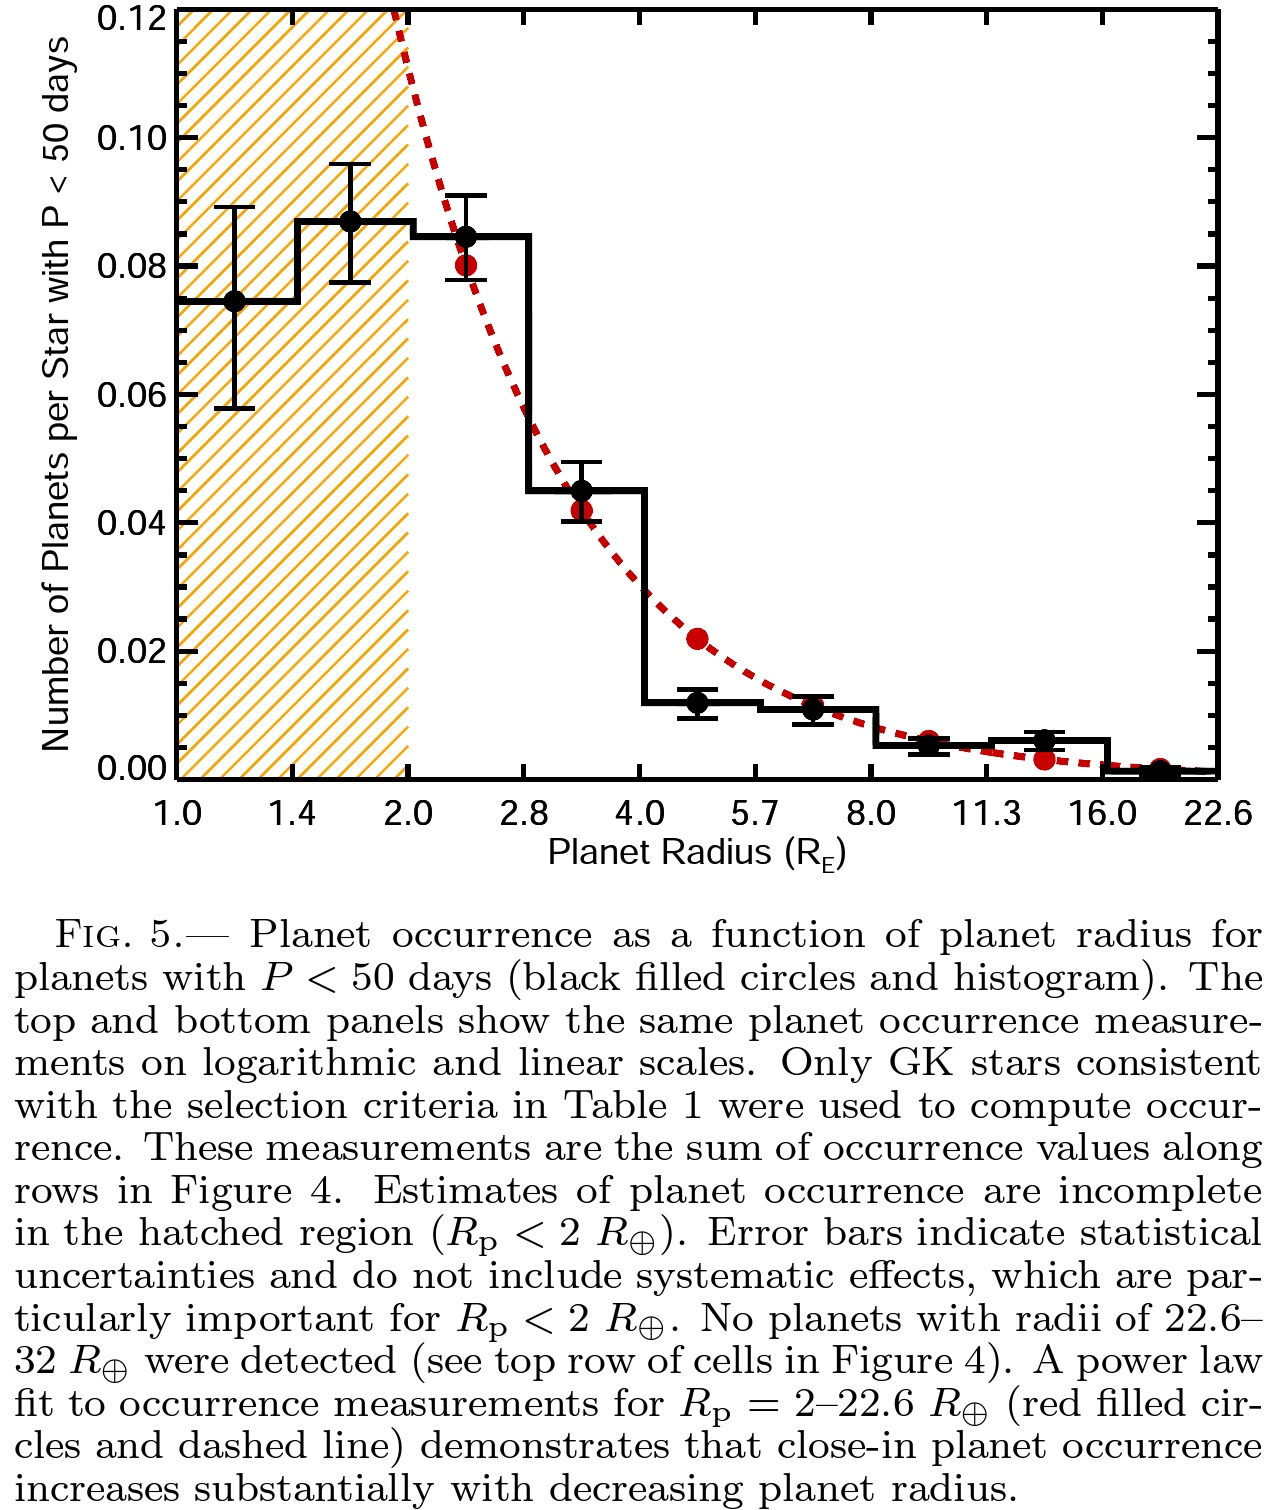
\includegraphics[trim={0cm 0 0 0},clip, keepaspectratio,width=0.9\textwidth]{freqvsRpl50d}\label{fig:freqvsRpl50d}\caption{Da \cite{}.}

\begin{figure}[!ht] \begin{subfigure}[b]{0.45\textwidth} \centering 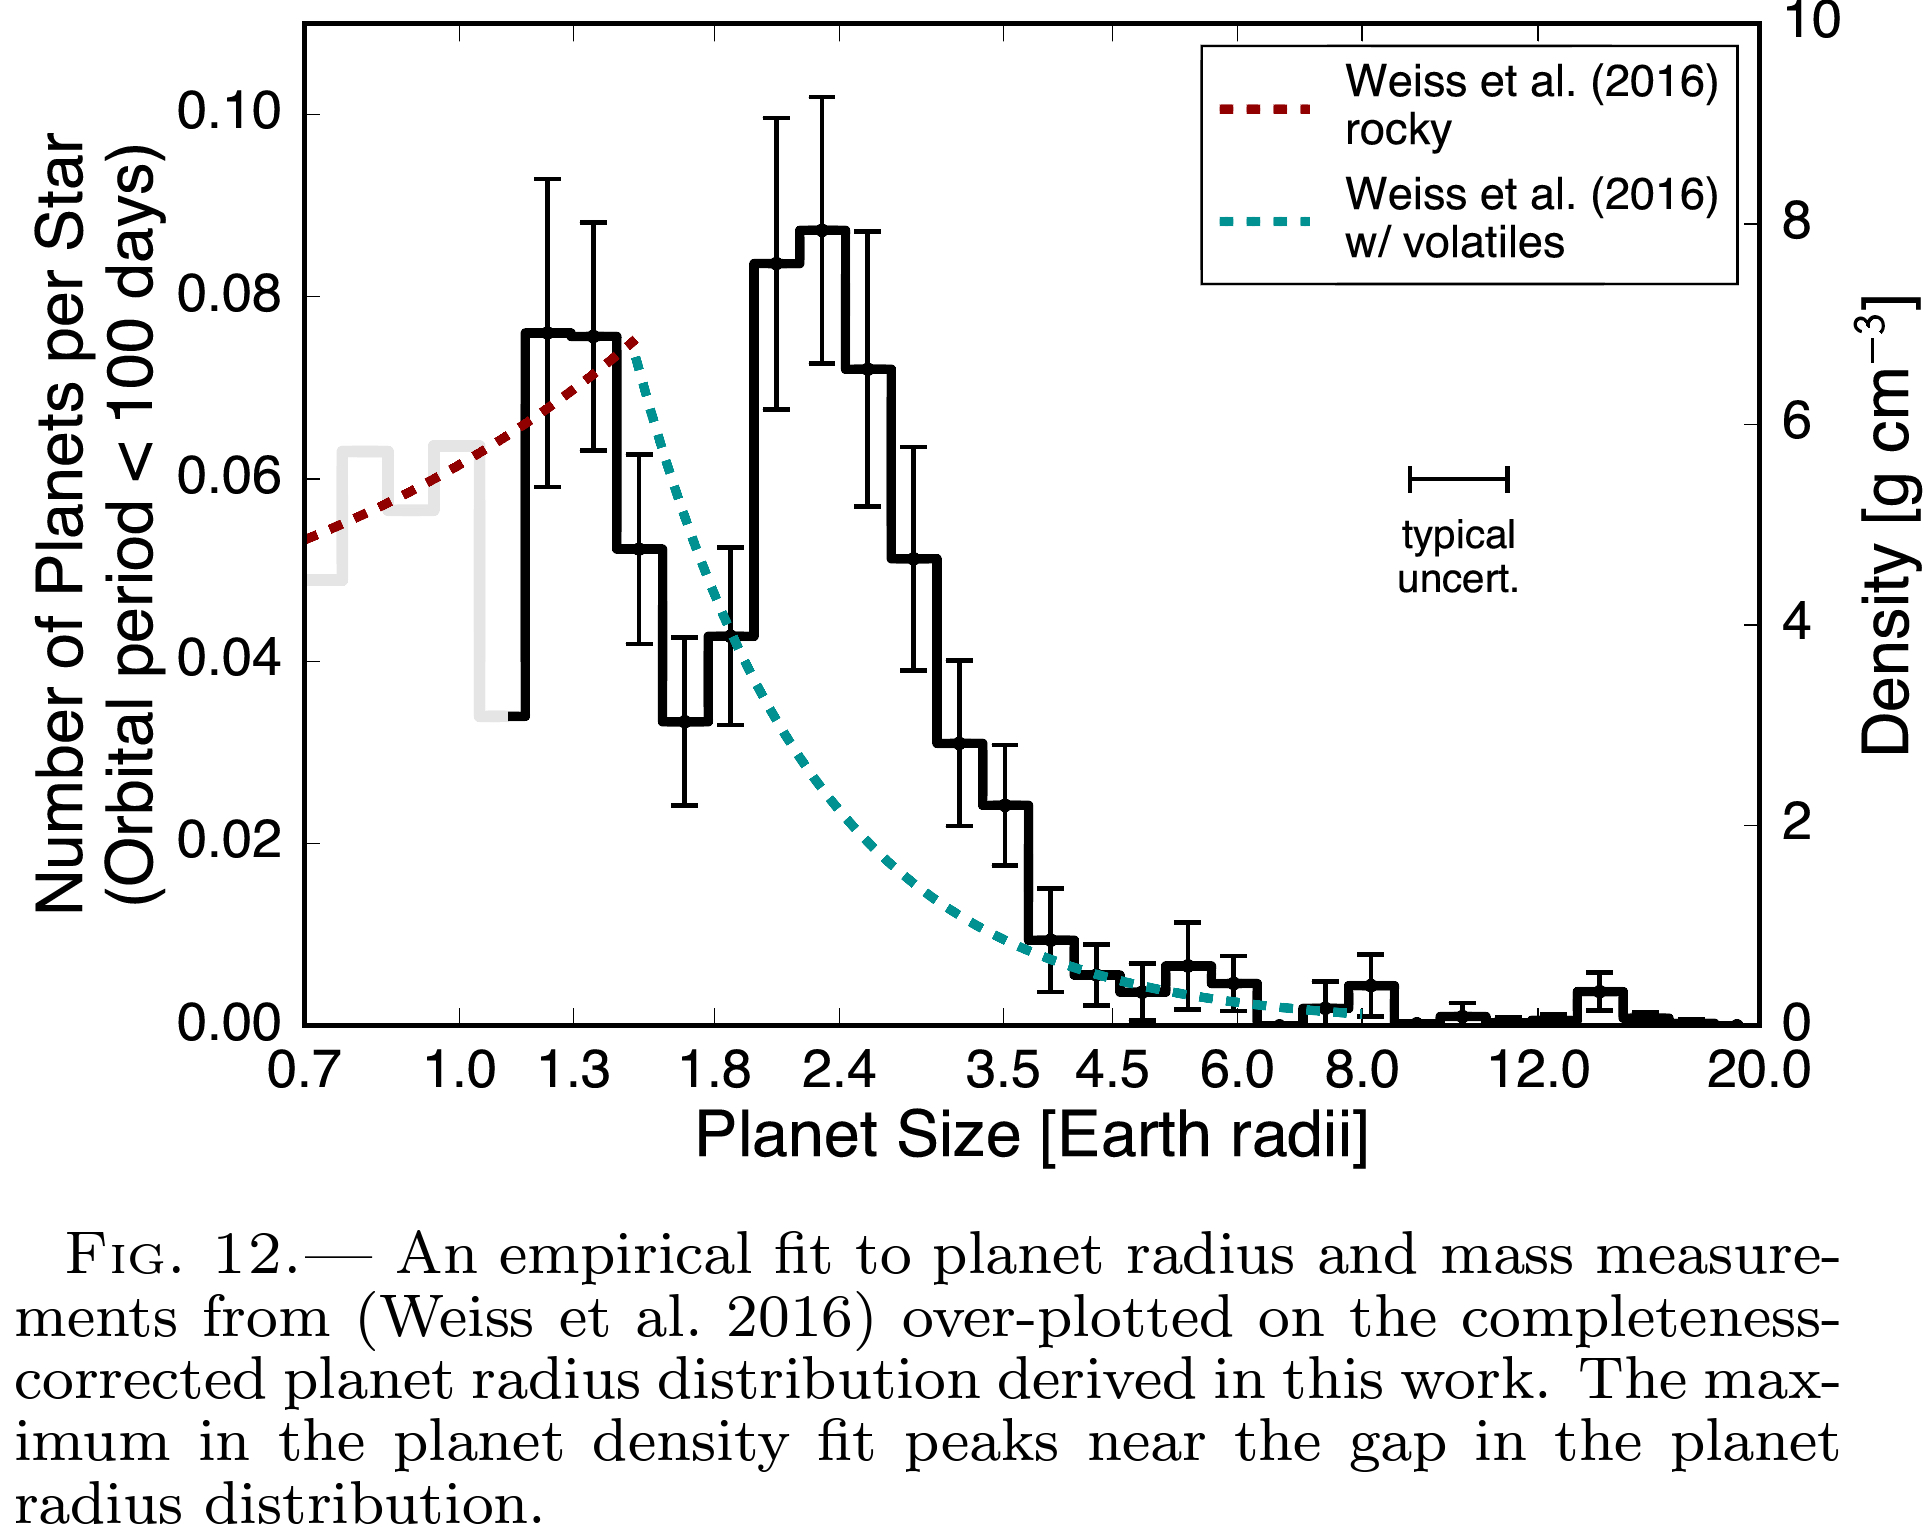
\includegraphics[trim={0 10cm 0 0},clip, width=0.95\textwidth]{RfreqPl100ub} 
\label{fig:RfreqPl100ub} \end{subfigure} ~ \begin{subfigure}[b]{0.55\textwidth} \centering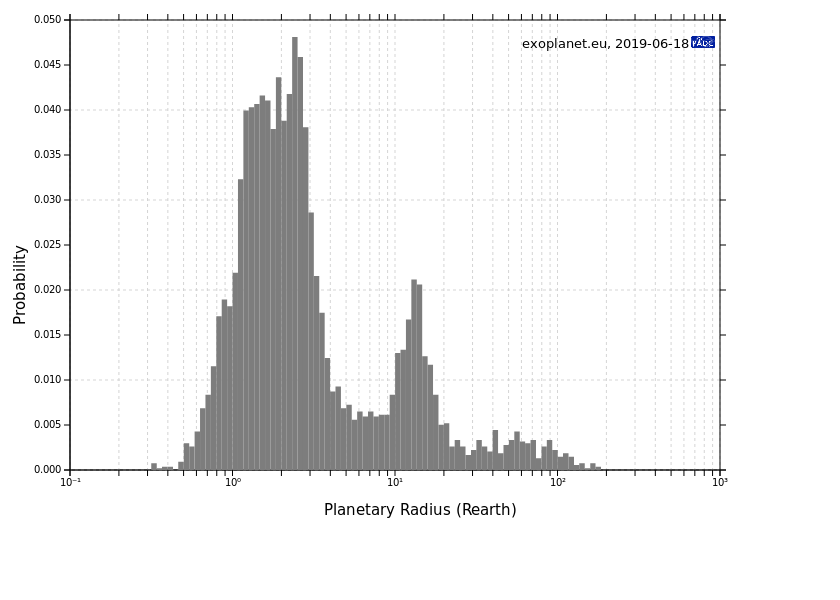
\includegraphics[trim={0cm 0 0 0},clip, keepaspectratio,width=0.9\textwidth]{Rfreq}\label{Rfreq}
 \end{subfigure}\caption{A sinistra: distribuzione per i pianeti osservati tramite transito con $P<\SI{100}{\day}$: il picco a $1.7\mearth{}$ si ipotizza causato dall'evaporazione. Da \cite{fulton2017california}. A destra: distribuzione radiale pianeti rivelati tramite T (da \cite{exoplanet.eu} (luglio 2018): la frequenza ha andamento crescente verso pianeti di raggio terrestre, andamento piatto tra $4-10\rearth{}$ e picco a $R\approx\rjupiter{}$.} \end{figure} 


\begin{workout}[transit distro observed refs]
Refs:Mthods of detecting exoplanets (radius distro: pg 136)
the occurrence within 0.25 au of solar-type stars from kepler
occurrence architecture exoplanetary
fressin 13: 
petigure 13: plateau PLANET POPULATION BELOW TWICE EARTH SIZE
bathala 13
exoplanet.eu
\end{workout}

\begin{workout}[radius distro]
Local maximum at $1\mjupiter{}$, flat distro in log(r) between $4-10\mearth{}$ below strong increase, at $1.7\mearth{}$ local minimum separating super-earth from sub-neptune
\end{workout}

\begin{workout}[planet model: relazione massa-raggio]
characterization of exoplanets from formation: MR relation pg 18
formazione: vedi \ref{ch:gasaccretion}
MR diagram chabrier 09 (perryman 143)

\end{workout}

La posizione di un pianeta nel diagramma massa-raggio \'e determinata dall'equazione di stato, e quindi da densit\'a e composizione. Per un equazione di stato della forma
\begin{equation}
P\propto\rho\expy{\gamma},\ \gamma=\frac{1}{n}+1
\end{equation}
si che per $M\approx\mjupiter$ $n\approx1$.
Inoltre la relazione massa-raggio  \'e approssimabile
\begin{equation}
R\propto M\expy{(1-n)/(3-n)}
\end{equation}•
Tramite un modello planetarie si ricava la composizione media di un pianeta dalla posizione nel diagramma mass-raggio.

\begin{figure}[!ht] \centering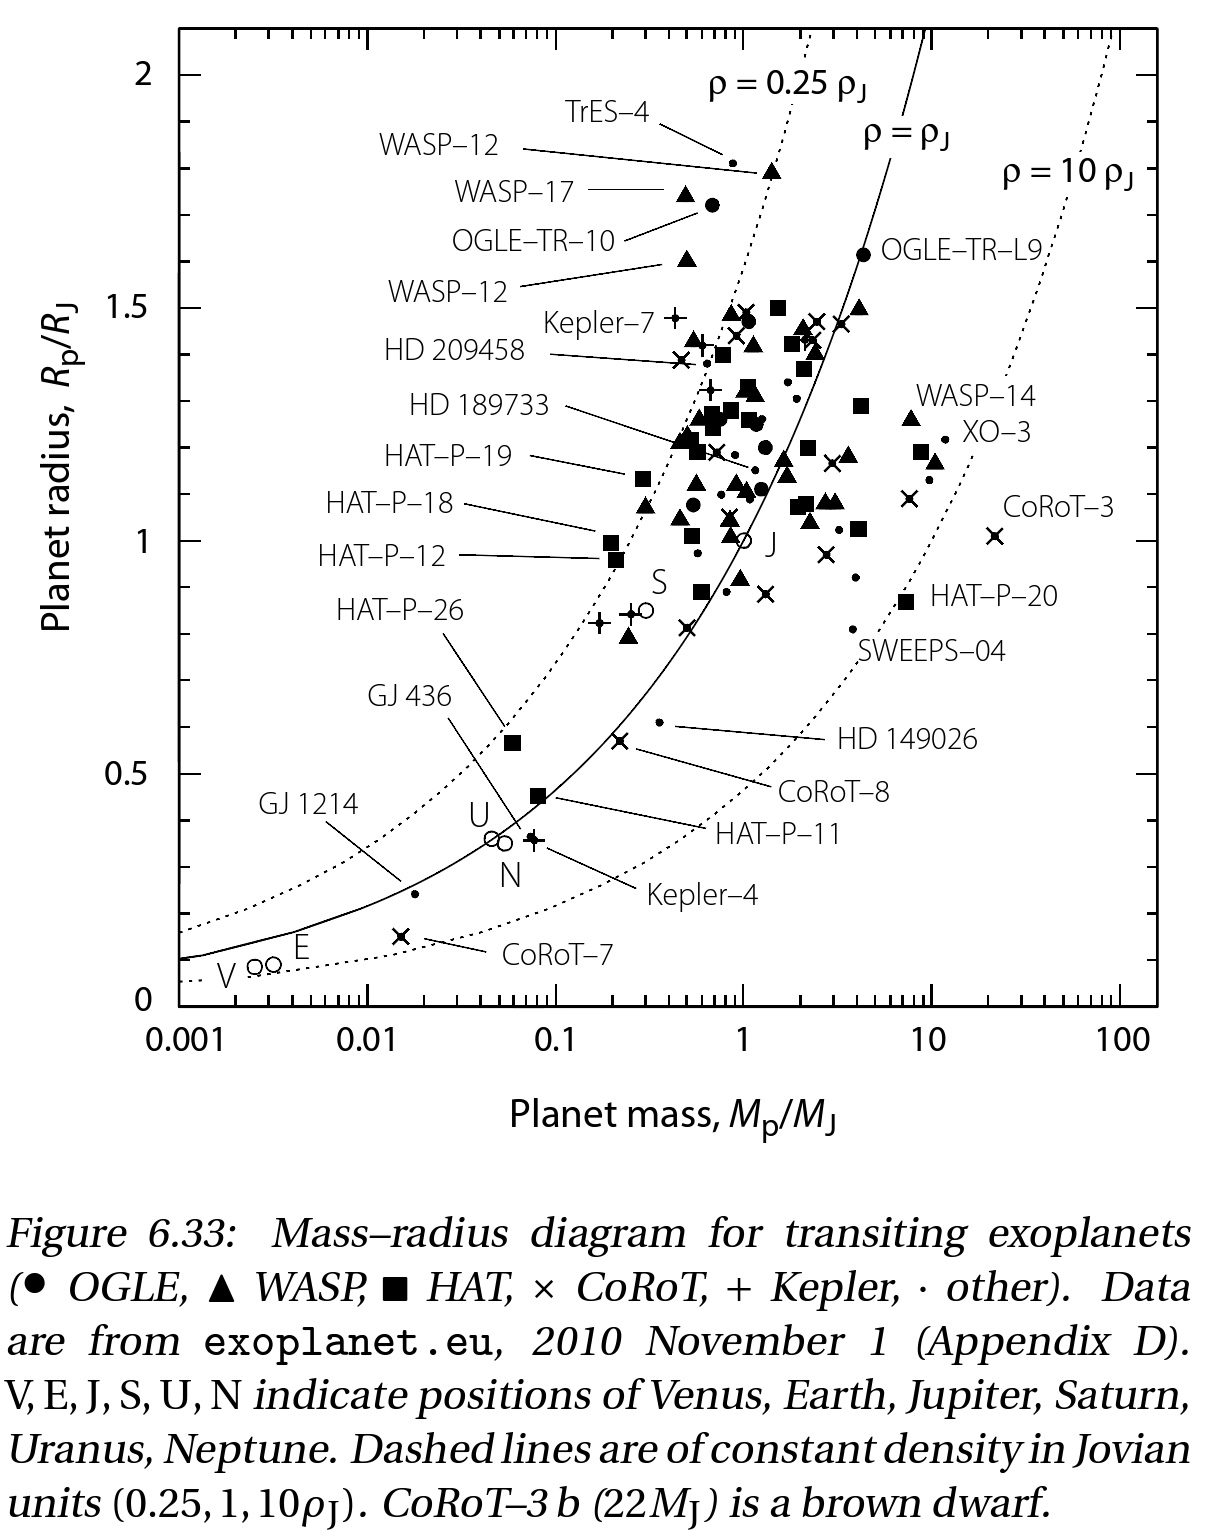
\includegraphics[trim={0cm 14cm 0 0},clip, keepaspectratio,width=0.9\textwidth]{MRD}\label{fig:MRD}\caption{Diagramma mass-raggio per pianeti di transito. Le curve tratteggiate sono a densit\'a costante. Il simbolo $\circ$ indica i pianeti del sistema solare. Da \cite{perryman2011exoplanet}.}
 \end{figure} 

\begin{workout}[KEPLER MULTI-PLANET SYSTEM]
THE CALIFORNIA-KEPLER SURVEY. V. PEAS IN A POD: PLANETS IN A KEPLER MULTI-PLANET SYSTEM ARE SIMILAR IN SIZE AND REGULARLY SPACED
						 III - A gap in radius distribution of small planets
\end{workout}

\begin{workout}[transiti refs: osservabilie probabilit\'a di rilevamento]
pg103
pg 117, eccentric orbit pg 121-122
From space: presence of structure on stellar surface Perryman 3.4, Eriksson Lindegren 07; simulation of stellar jitter: Svensson Ludwig 05, Ludwig 06.
Probability of randomlyoriented planet on circular/eccentric orbit (Borucki Summers 84/Barnes 07, Burke 08,  Seagroves 03, Kane von Braun 08):
\end{workout}

\begin{workout}[Transiti: Propriet\'a dei pianeti a transito]
pg 143, fig 6.33, 6.34, 6.35
Mass-radius relation: chabrier 09
\end{workout}

\begin{workout}[M-R diagram]
orbital migration 10.8 Perryman, tidal effect 10.9, 
fig11.2, 11,4 (EOS), 11.7, 11.8 (M-R)
Ternary diagram 11.9, M-R realtion
Fig 6.33/34/35: mass radius realtion

pg 144: theoretical model - La posizione di un pianeta nel diagramma M-R fornisce indicazione della composizione
fig 6.35
\end{workout}

\begin{workout}[Struttura orbitale e risonanze moto medio]
\end{workout}

\begin{workout}[Long term dynamical stability: mmr, fully packing, eccentricity, inclination distro]
tidal circularization
resonance capture and migration (pg 41)
barnes 08: secularly/resonant dominated
Planets near mmr (Petrovich 12): strength of resonance
P-P scattering leds to tightly packed planetary systems (Raymond barnes 09)
Architecture of planetary systems based om kepler data: number of planets and coplanarity (Fang Margot 12): e,i distro.
Spacing Kepler planets (Wu Pu 15)
Are planetary systems filled to capacity? (Fang Nargot 13)
\end{workout}
